Ever since the launch of the FCC conceptual design study in 2014, 
one of the primary objectives has been to design and develop a unified, 
synergistic, and adaptable software `ecosystem', 
to serve as a foundation for all future experiments at FCC-ee and FCC-hh. 
With its data processing framework and all the necessary tools 
inspired by the advanced software of running experiments and ongoing R\&D initiatives, 
the resulting ecosystem is aiming at addressing all future experiment's use cases, 
based on modern software technology. 
While this transformative approach required significant time to gain general acceptance, 
and even if the level of completeness is not anywhere close to that of running experiments, 
this new ecosystem is now regularly used by the FCC particle physicists in their daily work. 
The performance of some tools, such as flavour tagging algorithms, 
already far surpasses that of the algorithms used for past linear collider studies~\cite{ilcsoft}. 
Needless to say, further work is needed to fully enable all studies targeted by the FCC-ee scientific programme. 
For example, the following tasks (among many other necessary developments) 
were identified as priorities for the FCC Feasibility Study: 
\begin{itemize}

\item Proceed with the full and parametrised simulations (and their interplay) 
of the sub-detectors currently considered (Section~\ref{sec:concepts}), 
including digitisation and sub-detector interchange with a `plug-and-play' framework, 
towards enabling the study of the performance (Section~\ref{sec:requirements}) of a large variety of detector concepts.  

\item Develop and implement the various reconstruction and analysis tools for use by all collaborators, 
reaping the benefits from LHC experience and, whenever relevant, from past linear collider studies.

\item Complete the simulation of the interaction region,
also known as machine detector interface (MDI, Section~\ref{sec:mdi}),
in view of the final evaluation and mitigation of beam-related backgrounds in the detectors. 
This task includes streamlining the access to the Monte Carlo codes that simulate the relevant backgrounds.

\item Provide the technology needed to improve the accuracy of the simulation of beam-related quantities 
(such as the beam-energy spread, crossing-angle spread, bunch length and transverse size, 
final state particle deflection by the colliding bunches, etc.) 
as well as initial state and final state radiation (and their interference) 
to match the statistical precision expected at FCC-ee, in particular at the \PZ pole. 
Ensure that these technologies are usable in all Monte Carlo generator codes relevant for FCC-ee, 
in close interaction with the code authors.

\item Continue to drive the development of the common software framework (\textsc{Key4hep}) 
and common data format (\textsc{edm4hep}), 
ensuring that they meet the requirements of FCC, 
both in terms of functionality and of infrastructure building, testing and deployment.

\item Evaluate the need for computing resources and proceed with regular simulated data production. 
The computing needs for FCC-ee are dominated by the \PZ-pole run, both online and offline.
The corresponding demands are significant, even when compared to HL-LHC. 
By the time FCC-ee operations start, 
it will be crucial to leverage the advances and insights gained from HL-LHC, 
also in terms of resource sustainability. 
Even during the next phase of the study, 
the needs for fully simulated and reconstructed event samples, and for their analysis, 
are potentially challenging and require detailed identification, evaluation, and purchase of the necessary computing resources. 
Coordination with resource providers, which include CERN, WLCG grid sites involved in FCC research, and HPC centres, 
is required to identify ways to guarantee access to these resources.

\item Last but not least, 
provide the users with detailed documentation and regular pedagogical tutorials, 
as has been the case in the past decade.

\end{itemize}

This chapter reviews the progress made towards achieving the tasks listed above. 
The results presented and discussed reflect the collaborative efforts of the `Software and Computing work package', 
in conjunction with other work packages within the FCC PED feasibility study. 
A key factor in this progress has been the strong software core team at CERN, 
which provides the overall vision, delivers the daily technical coordination, 
and ensures the timely development of essential common tools.

\subsection{The FCC software ecosystem}
\label{sec:fsr_software}

During the FCC feasibility study, 
the focus has been to deliver the components deemed essential to meet the challenges of FCC-ee 
and to assess the physics potential of the proposed experimental infrastructure: 
a comprehensive suite of $\epem$ event and beam-background generators; 
a proper handling of the complex interaction region and associated backgrounds; 
an infrastructure that facilitated the implementation of detector subsystems and detector concepts
(i.e., their geometries, their simulation, and the development of versatile reconstruction algorithms); 
and tools for event analysis, visualisation, and resource management. 
The corresponding workflows are illustrated in Fig.~\ref{fig:workflows}. 

\begin{figure}[ht]
\centering
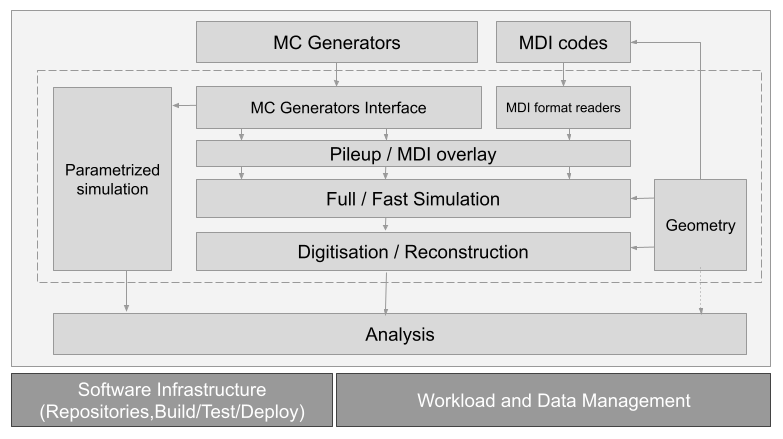
\includegraphics[width=0.8\textwidth]{Physics/SoftwareAndComputing/Figs/software-workflows.png}
\caption{Workflows to be supported during the project design and FCC Feasibility Study.}
\label{fig:workflows}
\end{figure}

Because this ambitious plan required human resources far beyond those available during this phase of the project, 
a proposal was made to other $\epem$ particle physicist communities to join forces 
and explore the possibility of developing a common software solution 
that could be adapted to the needs of all collider and detector geometries. 
Based on the initial FCC software framework developed during the Conceptual Design Study, nicknamed \textsc{fccsw}, 
and driven by the belief that the high-energy physics community was ready to 
further expand the number and role of shared components between experiments, 
the \textsc{Key4hep} initiative was launched after two founding workshops held in 2019 and early 2020~\cite{kickBO,kickHK}. 

Like any other large-scale software development, \textsc{Key4hep} is inherently a collaborative effort.
It builds on the experience of the LHC experiments, 
is integrated with community R\&D projects, 
and maximises the reuse of established solutions and packages, 
allowing experiments to benefit from existing community developments.  
Notable examples include the common core framework \textsc{Gaudi}~\cite{Gaudi}), 
developed and used by LHCb and ATLAS following the positive experience of BELLE,
the \textsc{dd4hep}~\cite{dd4hep} R\&D project for detector geometry, 
and other well-known packages like \textsc{Root}~\cite{root}, \textsc{Geant4}~\cite{Geant4}, or \textsc{Podio}~\cite{Podio}. 
By leveraging and contributing to these experiment-independent software packages, 
the \textsc{Key4hep} initiative aims at fostering a broader ecosystem of HEP software,  
enhancing collaboration and innovation across the field.

After recalling the main concepts of \textsc{Key4hep} in Section~\ref{sec:k4h}, the current status in each of the main areas is summarised in the following sections: common event data model (Section~\ref{sec:edm4hep}); event generators (Section~\ref{sec:generators}); parametrised (Section~\ref{sec:delphes}) and full (Section~\ref{sec:geometries}) simulation;  digitisation (Section~\ref{sec:digi}) and reconstruction (Section~\ref{sec:reco});  event analysis (Section~\ref{sec:analyses}); visualisation (Section~\ref{sec:visualisation}); and resources (Section~\ref{sec:resource}).

\subsection{The main components of \textsc{Key4hep}}
\label{sec:k4h}

The \textsc{Key4hep} ecosystem has been designed to address core requirements common to all experiments in a sufficiently robust manner, 
while allowing specific extensions to meet individual demands. 
High-energy physics data processing consists of several basic components that need to be chosen carefully, 
the most important of which are listed below.

\begin{enumerate}

\item A data processing framework provides the structure for integrating and steering all other components. 
For example, past linear collider studies used the \textsc{Marlin}~\cite{Marlin} framework for many years. 
In \textsc{Key4hep}, \textsc{Gaudi}~\cite{Gaudi} was chosen because of 
its widespread adoption by the LHC experiments,
its broader user and developer communities, 
and its recognised potential for future evolution, 
which includes support for accessing heterogeneous resources, 
accommodating different architectures, and enabling task-oriented concurrency.

\item A detector geometry description tool, 
chosen to be \textsc{dd4hep}~\cite{dd4hep} because of its already widespread use in the relevant communities. 
In addition to providing a comprehensive detector description for event simulation, reconstruction, and analysis, 
\textsc{dd4hep} is now also used in production by the CMS and LHCb collaborations. 
This adoption drives a consolidation and development process that is highly advantageous for future experiments, 
in particular in critical areas, such as alignment and calibration.

\item A common event data model, called \textsc{edm4hep} (Section~\ref{sec:edm4hep}).

\item An infrastructure to build, test, and deploy the required software with minimal effort, 
automating the installation and ensuring a consistently linked set of packages with correct dependency resolution. 
The LHC Collaborations addressed this challenge independently, without converging on a unified solution. 
The HEP Software Foundation's packaging working group identified the scientific package manager \textsc{Spack}~\cite{Spack} 
as a potentially promising common solution worth further exploration for use in HEP. 
In line with the \textsc{Key4hep} philosophy, 
\textsc{Spack} was evaluated and successfully used to build \textsc{Key4hep}, 
despite certain limitations~\cite{SPack-CHEP2024-K4H}. 
These challenges include limited support for development workflows and deployment capabilities, 
requiring custom in-house workarounds, 
such as those required to deploy build artifacts on \textsc{CernVM-FS}, 
the widely-adopted technology for software distribution in HEP.

\end{enumerate}

\subsection{The event data model \textsc{edm4hep}}
\label{sec:edm4hep}

The event data model defines the structures needed to describe the required event information in the persistent store. 
While, in principle, this model can be different from what is used in the transient store seen by the data processing algorithms, 
and also from algorithm to algorithm, 
adopting the same event model everywhere reduces the need for conversions, enhances generality, and improves interoperability.

Since the launch of the FCC studies, the choice has been for an event data model managed by \textsc{Podio}~\cite{Podio}, 
a toolkit that generates the data model implementation from templates. 
With this choice, the high-level description in YAML files using Plain-Old-Data (POD) simple types 
are separated from the low-level persistency layer, which can be optimised according to the back-end. 
Once the required classes are defined in the YAML file, the \textsc{Podio} tool creates the source code automatically. 
The same technology has been chosen for \textsc{Key4hep}, with an event data model referred to as \textsc{edm4hep}, 
initially based on the event data models used in past linear collider studies (\textsc{lcio}~\cite{lcio}) 
and in the FCC conceptual studies (\textsc{fccedm}~\cite{fcc-ee-cdr}) classes, and improved from there as needed. 

The underlying assumption is that the same event data model can be used for all types of HEP experiments, 
which is well-suited to the integrated FCC programme, with a lepton collider followed by a hadron collider.
This requirement appears to be fulfilled by \textsc{edm4hep}, 
although a more definitive assessment will become available only when the FCC-hh investigations are extended to more use cases. 

\subsubsection{A specific use case: LEP data in \textsc{edm4hep}}
\label{sec:lepedm4hep}

In the context of the LEP data preservation efforts, an initiative has been launched to migrate those data to \textsc{edm4hep}, 
in a pioneering attempt to analyse these real, non-simulated data in the FCC software ecosystem. 
Beyond the clear advantage of preserving the ability to extract new scientific insights from LEP data for future generations, 
this effort has several key objectives relevant to FCC-ee. 
Most interestingly, LEP and FCC-ee share the same collision type and several centre-of-mass energies. 
This initiative therefore opens a unique opportunity to FCC physicists to gain hands-on experience with real data, 
thereby preparing them for future analyses within the FCC-ee scientific programme. 
It can also provide a platform to validate and improve simulation, reconstruction, and analysis tools, 
thus enhancing their reliability for future collider studies.

A preliminary migration feasibility study is currently underway with data from the ALEPH experiment. 
The project aims at establishing a conversion workflow that integrates both the experiment legacy software, 
executed within dedicated containers with the latest operating systems and validated by the experiment, 
and \textsc{Key4hep}-based applications. 
The initial approach involves extracting data at the analysis 
level\footnote{For ALEPH, the initial focus is on the MINI format~\cite{alephnumbers} 
however, the methodology under development is designed to be adaptable 
and could also be extended to the more comprehensive DST data format.} 
into an operating system-agnostic ASCII format, 
which can then be used to reconstruct the \textsc{edm4hep} structures for FCC analyses. 
Additionally, the project seeks to recreate a bookkeeping database containing relevant ALEPH metadata.

The status of the project was presented in the autumn of 2024~\cite{alephe4hdphep,alephe4hfccfrit}.
The current findings provide encouraging evidence of the overall feasibility of the approach,
despite difficulties in recovering comprehensive documentation, 
retrieving detailed information about the data that are often hardcoded within the legacy software,
and reconstructing detailed metadata about the data samples. 
These findings highlight the importance of generalising this effort as part of a more structured and systematic project.
 
\subsection{Integration of event generators}
\label{sec:generators}

Event generators are a crucial component of the software infrastructure in any HEP experiment, 
to design optimal data analysis strategies, evaluate detector performance requirements, 
and compare them with the response of different detector solutions, 
ultimately maximising the physics potential of the project. 
The richness of the FCC physics programme introduces new challenges for event generators across multiple dimensions. 
The unprecedented statistical precision expected at the \PZ pole for FCC-ee,
and the expanded energy range of FCC-ee and FCC-hh, 
call for substantial theoretical advances (Section~\ref{sec:theory}). 
These very precise calculations need to be translated into similarly accurate, computationally efficient, 
and easily maintainable software packages. 

Many event generators are already included in \textsc{Key4hep}. 
The first set of event generators was derived from the `LCG stacks', 
i.e., software stacks developed and maintained in the EP-SFT group at CERN targeting the cases of ATLAS and LHCb.
These stacks are, however, more and more used by non-LHC projects, 
and have been progressively expanded to include event generators not used at the LHC, 
such as \textsc{Whizard}~\cite{whizard}, a general purpose event generator used for past linear collider studies. 
Today, \textsc{Key4hep} includes an extended set of generic event generators, 
able to cover most of the initial needs of future projects, 
such as \textsc{Pythia8}~\cite{pythia8}. 

The increasing interest for FCC-ee has brought in the need for more specific and more accurate event generators. 
State-of-art generators for high-energy $\epem$ collisions, however, date from the LEP era and have been minimally maintained since. 
One of the first tasks to be addressed in the FCC feasibility study was the recovery of the 
still very relevant LEP event generators, 
such as \textsc{kkmc}~\cite{Jadach:2022mbe}, \textsc{bhlumi}~\cite{bhlumi}, and \textsc{BabaYaga}~\cite{babayaga}. 
The generators and related tools available in \textsc{Key4hep} at the time of writing are listed in Table~\ref{tab:genlist}.

\begin{table}[ht]
\centering
\caption{List of generators and related tools available in \textsc{Key4hep} at the time of writing. 
Most of the generators are available in the upstream \textsc{Spack} repository; 
the ones added by the \textsc{Key4hep-Spack} repository are indicated with an asterisk.}
\label{tab:genlist}
\begin{tabular}{cccccc}
\toprule
\multicolumn{6}{c}{Generators} \\ \midrule
\textsc{BabaYaga}* & \textsc{baurmc} & \textsc{bhlumi}* & \textsc{crmc} & \textsc{EvtGen} & \textsc{Genie} \\
\textsc{Gosam} & \textsc{Guinea-pig}* & \textsc{Herwig3} & \textsc{Herwigpp} & \textsc{kkmc}* & \textsc{MadGraph5amc} \\
\textsc{Photos} & \textsc{Pythia6} & \textsc{Pythia8} & \textsc{Sherpa} & \textsc{Starlight} & \textsc{Superchic} \\
\textsc{Tauola} & \textsc{vbfnlo} & \textsc{Whizard} &  & & \\ \toprule
\multicolumn{6}{c}{Generator tools} \\ \midrule
\textsc{agile} & \textsc{alpgen} & \textsc{ampt} & \textsc{apfel} & \textsc{ccs-qcd} & \textsc{chaplin} \\
\textsc{collier} & \textsc{cuba} & \textsc{dire} & \textsc{feynhiggs} & \textsc{form} & \textsc{HepMC} \\
\textsc{HepMC3} & \textsc{heppdt} & \textsc{hoppet} & \textsc{hztool} & \textsc{lhapdf} & \textsc{lhapdfsets} \\
\textsc{looptools} & \textsc{openloops} & \textsc{professor} & \textsc{prophecy4f} & \textsc{qd} & \textsc{qgraf} \\
\textsc{recola} & \textsc{rivet} & \textsc{syscalc} & \textsc{thepeg} & \textsc{unigen} & \textsc{yoda} \\
\bottomrule
\end{tabular}
\end{table}

\subsubsection{Event generators as packages}

Within the software ecosystem, generators are software packages that come with their own build, test, and deploy recipes. 
The recipes allow \textsc{Key4hep} to build in share installation mode, run the built-in test programs, 
and install the binaries into a distributed shared file system (CernVM-FS).

The generated events need to be injected into the simulation workflow, 
which requires a low level of interoperability between the event generator and the rest of the chain, 
named \emph{Common Data Formats}.
This level ensures that the applications exchange information files that are understood by all relevant processes, 
even on different hardware.\footnote{Passing information through files might impact performance. 
However, reading Monte Carlo events from files is not a limiting factor at the LHC and will likely not be at FCC either.}
The event generators are indeed typically stand-alone applications producing files with the generated events, 
in ASCII or binary data format. 
These event data formats have evolved in time following the requirements set by the community and are briefly reviewed in the next section. 
Some recent event generators offer enhanced interoperability with \emph{Callable Interfaces}, 
i.e., an API of functions streamlining the exchange of information among various components and increasing flexibility. 
These APIs can also be used as interface to a framework, as is described in the next section. 

\subsubsection{Common data formats}

The data formats produced by event generators provide structures to store the lists of particles per event, 
with their momenta and type, information relevant to the event, such as its weight(s), 
and information relevant to the run, such as the configuration and version of the generator. 
Several formats serving similar purposes appeared in the years ahead of the LHC. 
Among these, \textsc{StdHep}~\cite{stdhep} and \textsc{HepEvt}~\cite{hepevt} are first attempts to create standards, 
a challenge that has been assumed by \textsc{HepMC}~\cite{hepMC}, 
the latest version of which (version~3) includes readers for most of the available formats. 
The complexity of the generators developed for LHC brought in new needs, 
essentially to store information about matrix elements and alike. 
They have been included in the `Les Houches Event format' (LHEf). 
This format had initially been designed to transfer the matrix-element information to the parton shower component, 
but has since been used as a generic format at LHC and beyond, including FCC.

To handle the plethora of formats, 
\textsc{Key4hep} ensures that readers for all the formats required by the event generators of interest 
are available for all the simulation chains in use, based either on \textsc{Gaudi} or with standalone applications. 
For \textsc{Gaudi} applications, 
such as those using the framework components provided by \textsc{k4SimDelphes}~\cite{k4simdelphes} 
and/or \textsc{k4SimGeant4}~\cite{k4simgeant4}, 
the readers are implemented as \textsc{Gaudi} algorithms 
and transform the input from the files into \textsc{edm4hep} structures in memory 
that can be parsed by the next simulation algorithm. 
For standalone applications, 
such as those provided by \textsc{k4SimDelphes} (Section~\ref{sec:delphes}) or \textsc{DDsim} (Section~\ref{sec:geometryStrategy}), 
support for the formats is implemented within the applications.  

In the context of the ongoing ECFA activities for electroweak and Higgs factories, 
the \textsc{HepMC3} and \textsc{edm4hep} formats were recommended for the next versions of event generators, 
and the latter is deemed more suitable to meet the needs of the community. 
These recommendations were discussed at a dedicated event in June 2024~\cite{mcsupporttoolsevt}.

\subsubsection{Configuration}

The configuration of generators for Monte Carlo simulations often involves redundant efforts, 
as different generators aim at the same physics processes. 
To streamline this process and improve efficiency, 
the \textsc{k4GeneratorConfig}~\cite{GenConfig} package provides a unified approach to generator inputs. 
The package, which is already included in \textsc{Key4hep}, addresses essentially two challenges: 
lack of standardisation 
(each generator requiring a specific input format despite simulating, in principle, the same physics processes), 
and author involvement 
(relying on authors to adopt a common input format is impractical, 
as they are unlikely to change existing workflows or agree on a unified approach).
The proposed solution consists in the creation of a master input card defining the required parameters and configuration for simulations, 
which is then converted by a dedicated Python module into generator-specific runcards, 
ensuring compatibility across different MC tools. 
This approach will automate the creation of inputs tailored to each generator while maintaining consistency with the master card.

The targetted benefits are reproducibility and error minimisation, 
as a unified configuration process inherently reduces discrepancies and manual errors in input preparation, 
and minimises the potential for mistakes that can arise from manual handling of generator-specific configuration cards. 
The solution also provides a way to improve legacy preservation, 
as the system also supports the older `LEP era generators', 
ensuring continued usability, even when there is no active development by the original authors.

An initial set of generators has already been integrated in the system 
and an infrastructure has been set up to enable running and comparing benchmarks of the tools. 
A status report was presented at the 3$^\text{rd}$ ECFA workshop, in October 2024~\cite{GenConfigECFAParis}.

\subsection{Parametrised simulation}
\label{sec:delphes}

The \textsc{Delphes} parametrised simulation toolkit~\cite{delphes} is integrated into \textsc{Key4hep}. 
By applying resolution and efficiency functions to generator-level objects, \textsc{Delphes} offers a high-level approximation of the detector response in a highly flexible and lightweight tool. Its capabilities encompass the propagation of charged (and neutral) particles in a magnetic field, the modelling of electromagnetic and hadronic calorimeters, and the parametrisation of muon identification efficiencies. 
Basic elements like charged-particle tracks and calorimeter energy clusters are reconstructed from the simulated detector response. A simplistic particle-flow reconstruction combines tracks and calorimeter information to form a list of particle candidates in a global event description. These particles are then used as input to form higher-level objects such as isolated leptons, jets, and total/missing energy and momentum.  Although the physics performance obtained from \textsc{Delphes} represents 
the best that could be achieved with nominal sub-detector resolutions, this tool shows a reasonable agreement with the more detailed full simulation, as discussed in Section~\ref{sec:PhysPerf_FullSim}, and can thus be used to establish detector requirements and to provide rather robust estimates of the FCC-ee physics potential.   

The \textsc{Delphes} toolkit was enhanced with several new features, which include an algorithm reconstructing the charged-particle track parameters and covariance matrix for arbitrary tracking geometries;  a module for deriving time-of-flight measurements; 
and a tool that parametrises the number of ionisation clusters associated with the trajectory of a charged particle in a gaseous detector, based on simulations from \textsc{Garfield}~\cite{garfield}. These tools have been incorporated into the central \textsc{Delphes} package and are employed, in particular, to train a graph neural network for jet flavour identification~\cite{flavorTaggingDelphes}. Illustrating distributions produced with these new modules are shown in Fig.~\ref{fig:pid_delphes}. 

\begin{figure}[ht]
\centering
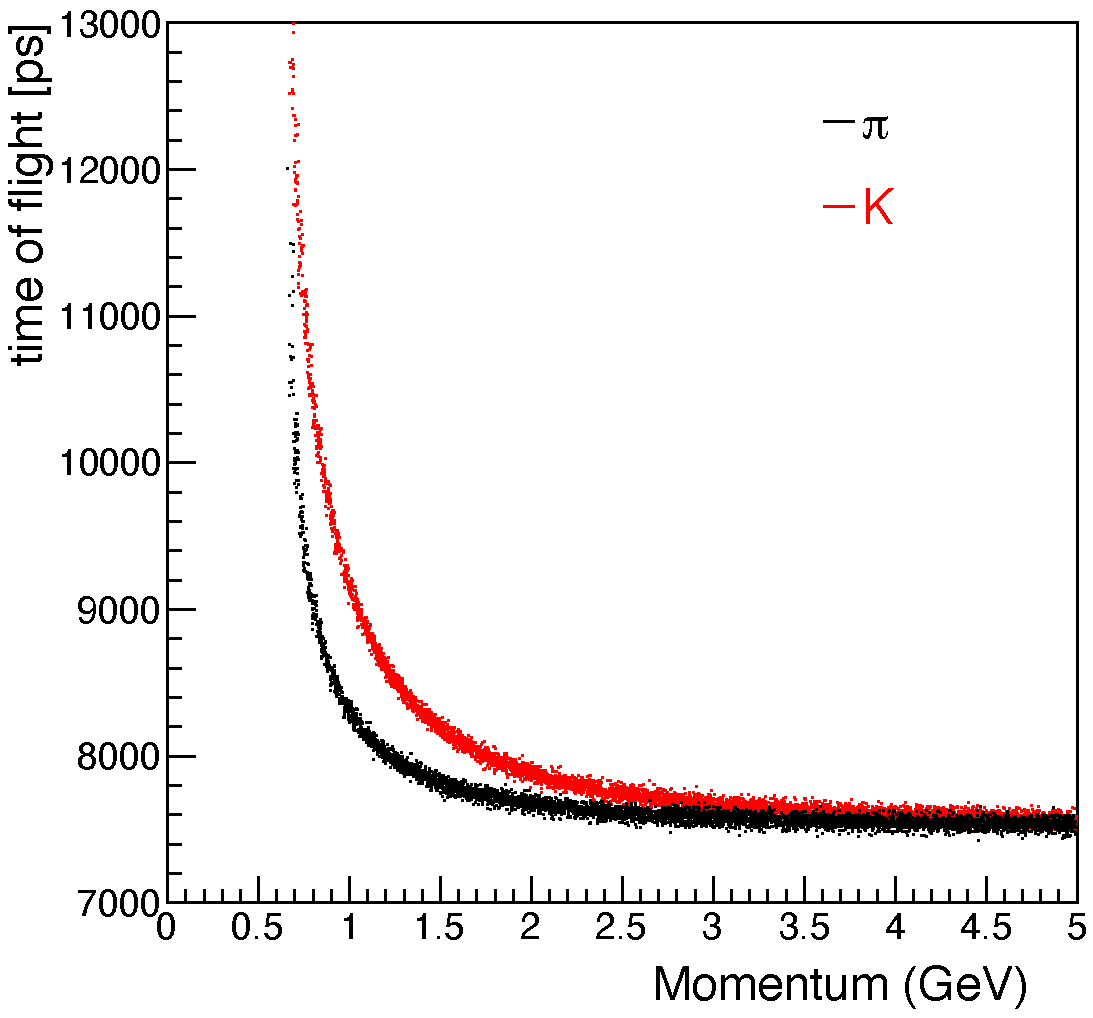
\includegraphics[width=0.32\columnwidth]{Physics/SoftwareAndComputing/Figs/tof-vs-p.pdf}
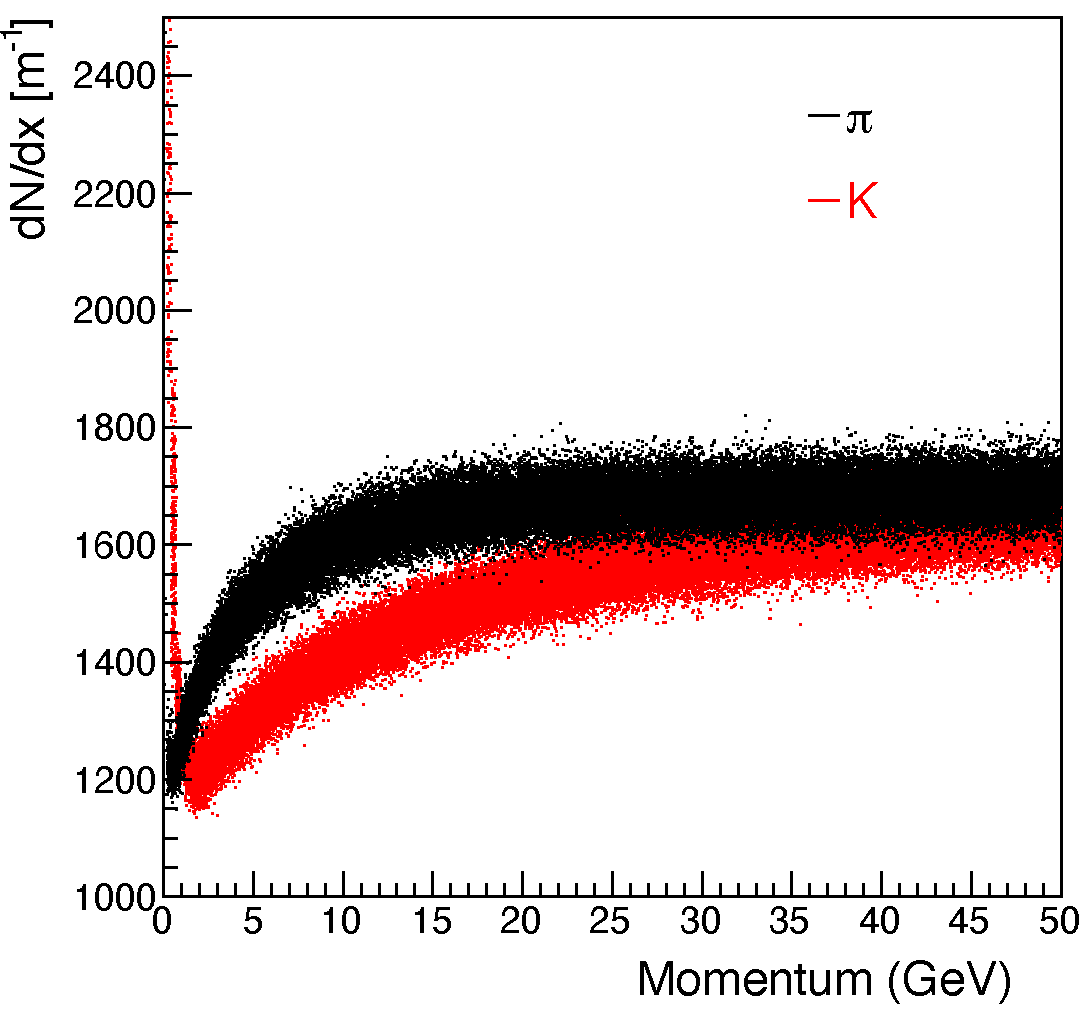
\includegraphics[width=0.32\columnwidth]{Physics/SoftwareAndComputing/Figs/dndx-vs-p.pdf}
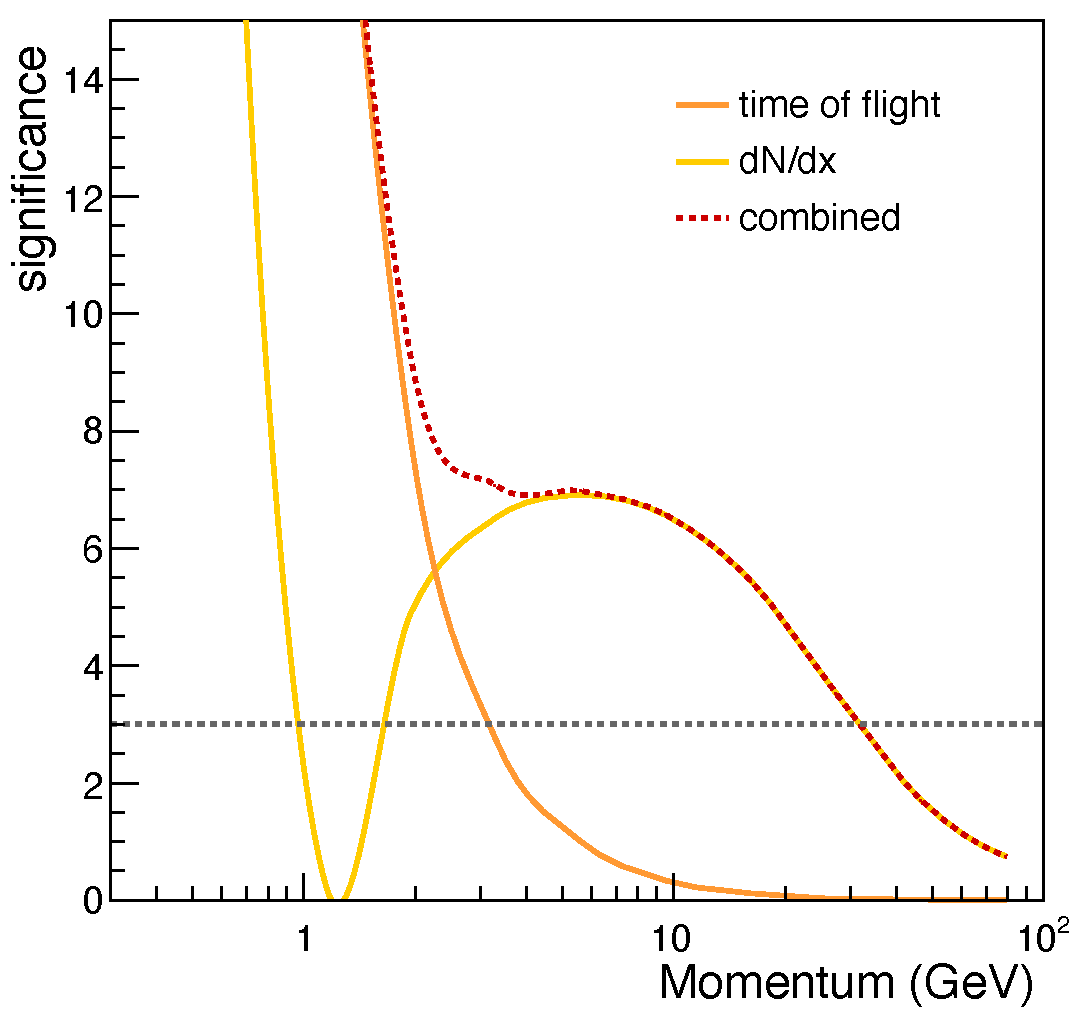
\includegraphics[width=0.32\columnwidth]{Physics/SoftwareAndComputing/Figs/comb_pid-vs-p.pdf}
\caption{Particle identification metrics for charged kaons and pions emitted at $\theta = 90\,^\circ$, 
as derived from the IDEA detector \textsc{Delphes} parametrisation. 
From left to right, the plots display, as a function of the particle momentum,
the time-of-flight in the tracker, 
the number of ionisation clusters per unit length for a gas mixture of 90\% He and 10\% Isobutane, 
and their respective or combined separation power in terms of standard deviations.}
\label{fig:pid_delphes}
\end{figure}

A \textsc{Delphes} configuration card simulating the expected performance of the IDEA detector concept, 
with a detailed layer-by-layer description of its tracking system, 
has been implemented and added to the central repository~\cite{delphes_card_idea}. 
An alternative version of this parametrisation, featuring a full silicon tracking system, 
was also developed to emulate physics performance closer to what is anticipated from the CLD detector concept. 
The integration of CLD calorimeter parametrisations into this card is under development. 
More information on these parametrisations can be found in Ref.~\cite{softwareNote}.

The \textsc{Delphes} integration into \textsc{Key4hep} is achieved through the \textsc{k4SimDelphes} package~\cite{k4simdelphes}, which wraps the core components of \textsc{Delphes} and adds the functionality to convert its output into the \textsc{edm4hep} data model. 
Several command-line tools (\textsc{Delphes*\_edm4hep}) simplify the use of these extensions in stand-alone mode, 
while the \textsc{k4SimDelphesAlg} \textsc{Gaudi} algorithm enables full integration of \textsc{Delphes} simulations 
within a \textsc{Key4hep} workflow, 
allowing users to benefit from features such as the generator functionalities described in Section~\ref{sec:generators}. 

To enhance flavour physics studies in parametrised simulations, an interface between \textsc{Pythia8} and \textsc{EvtGen} is implemented, and is fully integrated with the \textsc{Delphes} applications. This interface enables efficient generation of background contributions in regions of phase space where specific signals are expected (e.g., rare hadron decays or long-lived particles). Users must apply a posteriori normalisations `manually' to ensure consistency between the generated number of events and the reported cross sections.

\subsection{Full simulation}
\label{sec:geometries}

Some applications require simulations with a higher level of detail than \textsc{Delphes}. For example, R\&D efforts and physics analyses that access detector-level information demand a more detailed description of the detector geometry and response. 
To address these needs (and, incidentally, to validate the detector parametrisation outlined in the previous section), a detailed modelling of all the (sub-)detectors considered for FCC is actively being developed. This section provides an overview of the current status of geometry implementation, along with existing examples of full detector configurations using different combinations of sub-detectors.

\subsubsection{Detector description and simulation strategy}
\label{sec:geometryStrategy}

The \textsc{dd4hep} toolkit~\cite{dd4hep} (Section~\ref{sec:k4h}) is used to model FCC detector geometries. 
This modern community standard hides the geometry complexity and allows high-level aspects 
(such as sub-detector dimensions, shape and materials, or the list of sub-detectors to be combined into a complete detector concept) 
to be configured by non-expert users with simple \textsc{xml} (`compact') files in a flexible plug-and-play approach, crucial for detector optimisation efforts.
This approach allows the optimisation of (sub-)detector variants without the need for recompilation and without an in-depth understanding of the technical details of the geometry implementation. 
It is essential, however, that the developer of the C++ detector builder (also called `detector driver') 
incorporates the necessary prescriptions and safeguards to ensure that a `sane' geometry be implemented under all circumstances. 
Several tools are available in \textsc{dd4hep} to validate the resulting geometries, such as checks to ensure that detector volumes do not overlap. 

While implementing a completely new sub-detector geometry is a more complex task, 
numerous examples and a wealth of community expertise greatly facilitate this process. 
Adding the newly created sub-detector to an existing concept, 
or building a new concept using existing sub-detectors, 
is straightforward using the `master' \textsc{xml} files that manage the list of sub-detectors and their envelope dimensions. 
This, again, assumes that the C++ drivers are designed to adapt dynamically to changes in outer envelope dimensions. 
A policy has been set in place to document \textsc{xml} parameters that require additional prescriptions before modification, 
complementing the sanity check tools to reduce the risk of creating ill-defined geometries.

The \textsc{dd4hep} framework is also well-suited for the modelling of individual modules used in test beams. 
Implementing test-beam geometries into this framework for the upcoming R\&D activities would be highly advantageous, 
as it would provide a basis for preparing complete sub-detectors, 
in view of their integration into full detector concepts. 
Occasionally, the availability of complete sub-detector geometries predates the test-beam campaigns. 
In such cases, R\&D teams could simplify and adapt the more complex full geometry to create the individual module.

The \textsc{Geant4} simulations are run on these models through the \textsc{ddSim} tool provided by \textsc{dd4hep}. 
This tool provides many functionalities that help the simulation configuration through command-line arguments or 
Python steering files (or a combination thereof), and can be run with simple particle guns or by providing input files containing the particles from Monte Carlo generators. 
Most common formats are supported: \textsc{HepMC(3)}, \textsc{HepEvt}, \textsc{StdHep}, 
and the so-called `pair' files produced by \textsc{GuineaPig++} 
(in addition to the \textsc{lcio} format). 
The output format can be \textsc{edm4hep}, \textsc{lcio}, or the \textsc{dd4hep} native format.

\subsubsection{Sub-detector models}
\label{sec:subdetectors}

Sub-detector geometries are available in the \textsc{k4geo} \textsc{gitHub} package~\cite{k4geo}.
The currently available \textsc{dd4hep} drivers, relevant for FCC-ee, are listed below. 
A more thorough description of their implementation details can be found in Ref.~\cite{softwareNote}.

\begin{itemize}

\item \textbf{Beam-pipe and related MDI components.} 
Two different models exist: one based on `native' \textsc{Geant4} shapes with a simplified geometry 
and the other exploiting the ability of \textsc{dd4hep} to directly import the CAD-based technical drawings, 
thus providing a much higher level of detail at the expense of poorer computing performance.

\item \textbf{Vertex detectors.} 
The driver used to model, for instance, the CLD vertex barrel detector, 
builds an arbitrary number of layers made of staves parallel to the $z$ axis with two different materials 
(one for the sensitive layers and the other for the support). 
The endcaps are constructed with simple octagonal plates perpendicular to the $z$ axis, 
made of an arbitrary number of slices with different thicknesses and materials. 
Another detector builder was recently developed to model the IDEA vertex detector. 
This driver offers a higher level of detail: 
it accounts for non-sensitive edges of the modules and includes staves/petals internal structures, together with support components. 
A switch in this driver allows the modelling of a geometry with almost support-free curved sensors.

\item \textbf{Main Trackers.}
Two versions are available: 
the former modelling a full silicon tracker, following an approach similar to that of the CLD vertex detector builder, described above, and the latter modelling a full stereo gaseous drift chamber. 
The latter features hyperboloid layers and twisted tubes to emulate the cell volume hosting the sense and field wires. 
The full geometry is built with a handful of user-provided parameters:
global dimensions, number of (super)layers, number of cells in the first layer and its increment from one layer to the next, etc. 
A third model, describing a straw-tube tracker, is under preparation.
    
\item \textbf{Dedicated particle identification detector.} 
A first version of the Array of RICH Cells (ARC) concept, described in Section~\ref{sec:concepts}, is implemented. 
The driver builds both the barrel and the endcaps, and omits, for now, the cells in the transition region, given their higher complexity. 
This detector builder includes the radiator gas and aerogel, the mirrors, the sensitive silicon sensors, 
the cooling plates and the outer vessel. 
The mirror positions and inclinations are set according to Ref.~\cite{Tat_ARC}. 
The material budget of the full sub-detector implementation corresponds to approximately 5\% of a radiation length and can be easily tuned.
    
\item \textbf{Calorimeters.} 
The following drivers are available: 
SiW luminosity calorimeter, 
noble liquid calorimeter with inclined absorber/readout planes, 
scintillating tile calorimeter (`tileCal'), 
and two fibre dual readout calorimeters, 
one with a capillary tube-based geometry and one where the fibres are directly inserted into metallic towers.
A detector driver modelling a segmented crystal-based dual readout calorimeter is being integrated in \textsc{Key4hep}. 
The simulation of dual readout calorimeters is especially challenging, 
in particular because of the number of scintillating photons generated, 
and requires special prescriptions~\cite{softwareNote}. 
The high-granularity calorimeters proposed for CLD are built with the generic driver described below.

\item \textbf{Generic detector builders.}
Some drivers have been designed generically to serve multiple purposes. 
For example, \textsc{GenericCalBarrel\_o1\_v01} and \textsc{GenericCalEndcap\_o1\_v01}, 
are used, e.g., to build the ECAL, HCAL, and muon system of CLD. 
These drivers arrange user-defined layer sequences, either radially or along the $z$-axis, 
forming a polyhedron with a customisable number of sides, set in the compact file.
Another example of a generic detector builder is \textsc{muonSystemMuRWell\_o1\_v01},
which defines stacks of layers made of user-defined tiles (e.g., PCB's)
and also provides flexibility on the number of sides, as illustrated in Fig.~\ref{fig:muRWELL}. 
This flexibility is an appealing feature at this stage of the project,
as it allows the software implementation to smoothly and rapidly adapt to detector R\&D choices. 
Unlike the formerly described drivers building the CLD calorimeters and muon system,
\textsc{muonSystemMuRWell\_o1\_v01} allows the user to define some overlap between the tiles 
(e.g., to account for their possibly non-sensitive edges) 
and stagger each side of the polyhedron to ensure a fully hermetic coverage.
This constructor is used to model the IDEA $\mu$RWELL-based muon system and pre-shower sub-dectectors. 

\end{itemize}

\begin{figure}[ht]
\centering
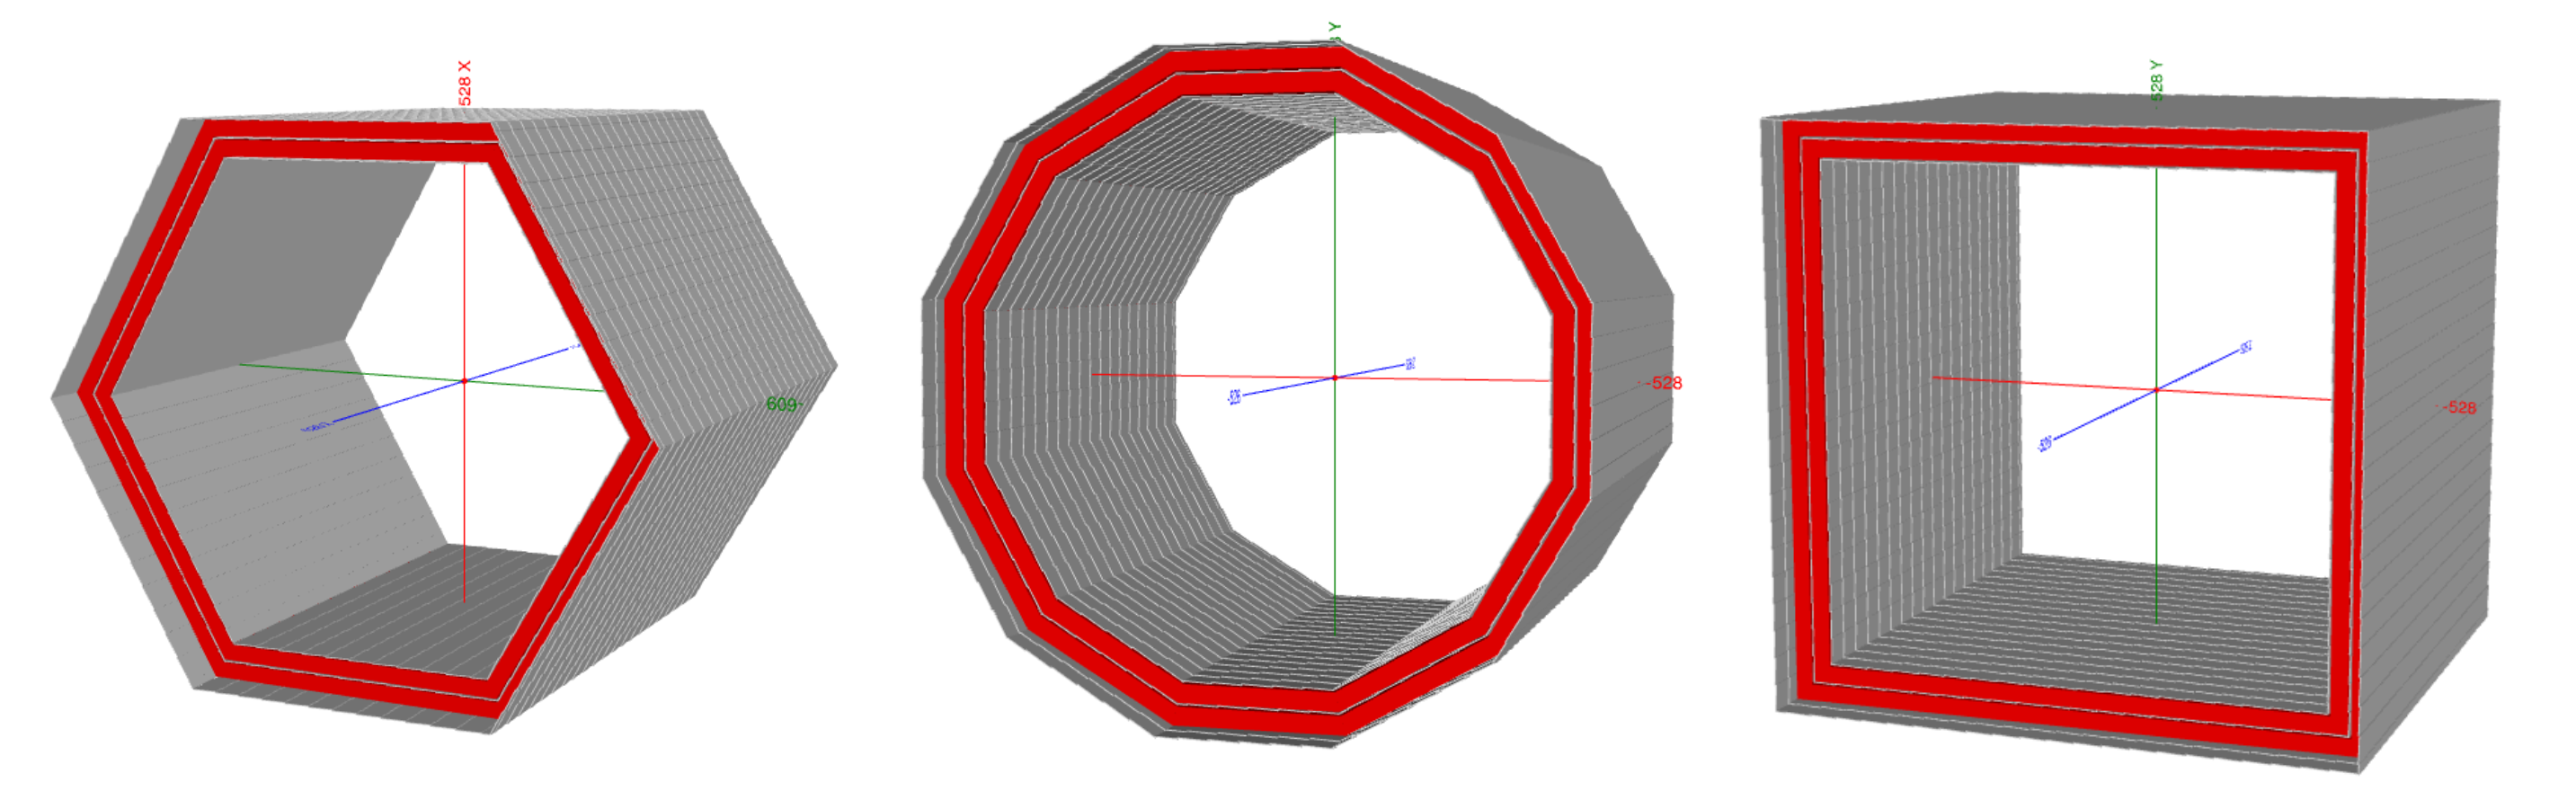
\includegraphics[width=\textwidth]{Physics/SoftwareAndComputing/Figs/Layered_polyhedron_overlap_shapes.png}
\caption{Illustration of the flexibility provided by the detector driver that builds $\mu$RWELL-based muon systems:
different barrel implementations with 6, 12, and 4 sides (from left to right). 
The grey layers represent the sensitive detector components, while the return yokes are shown in red.}
\label{fig:muRWELL}
\end{figure}

\subsubsection{Full detector models}

The availability of these sub-detector geometries along with the plug-and-play philosophy of \textsc{dd4hep} 
facilitates the creation and implementation of full detector concept alternatives. 
These models are hosted in the \textsc{k4geo} \textsc{gitHub} package~\cite{k4geo} 
and take the MDI components (beam-pipe, compensating solenoids, shields, LumiCal, etc.) 
from a central place, to ease the software maintenance. 
Pictures of three detector concepts, as they are currently implemented in \textsc{dd4hep}, 
are shown on Fig.~\ref{fig:threeDets}.

\begin{figure}[ht]
\centering
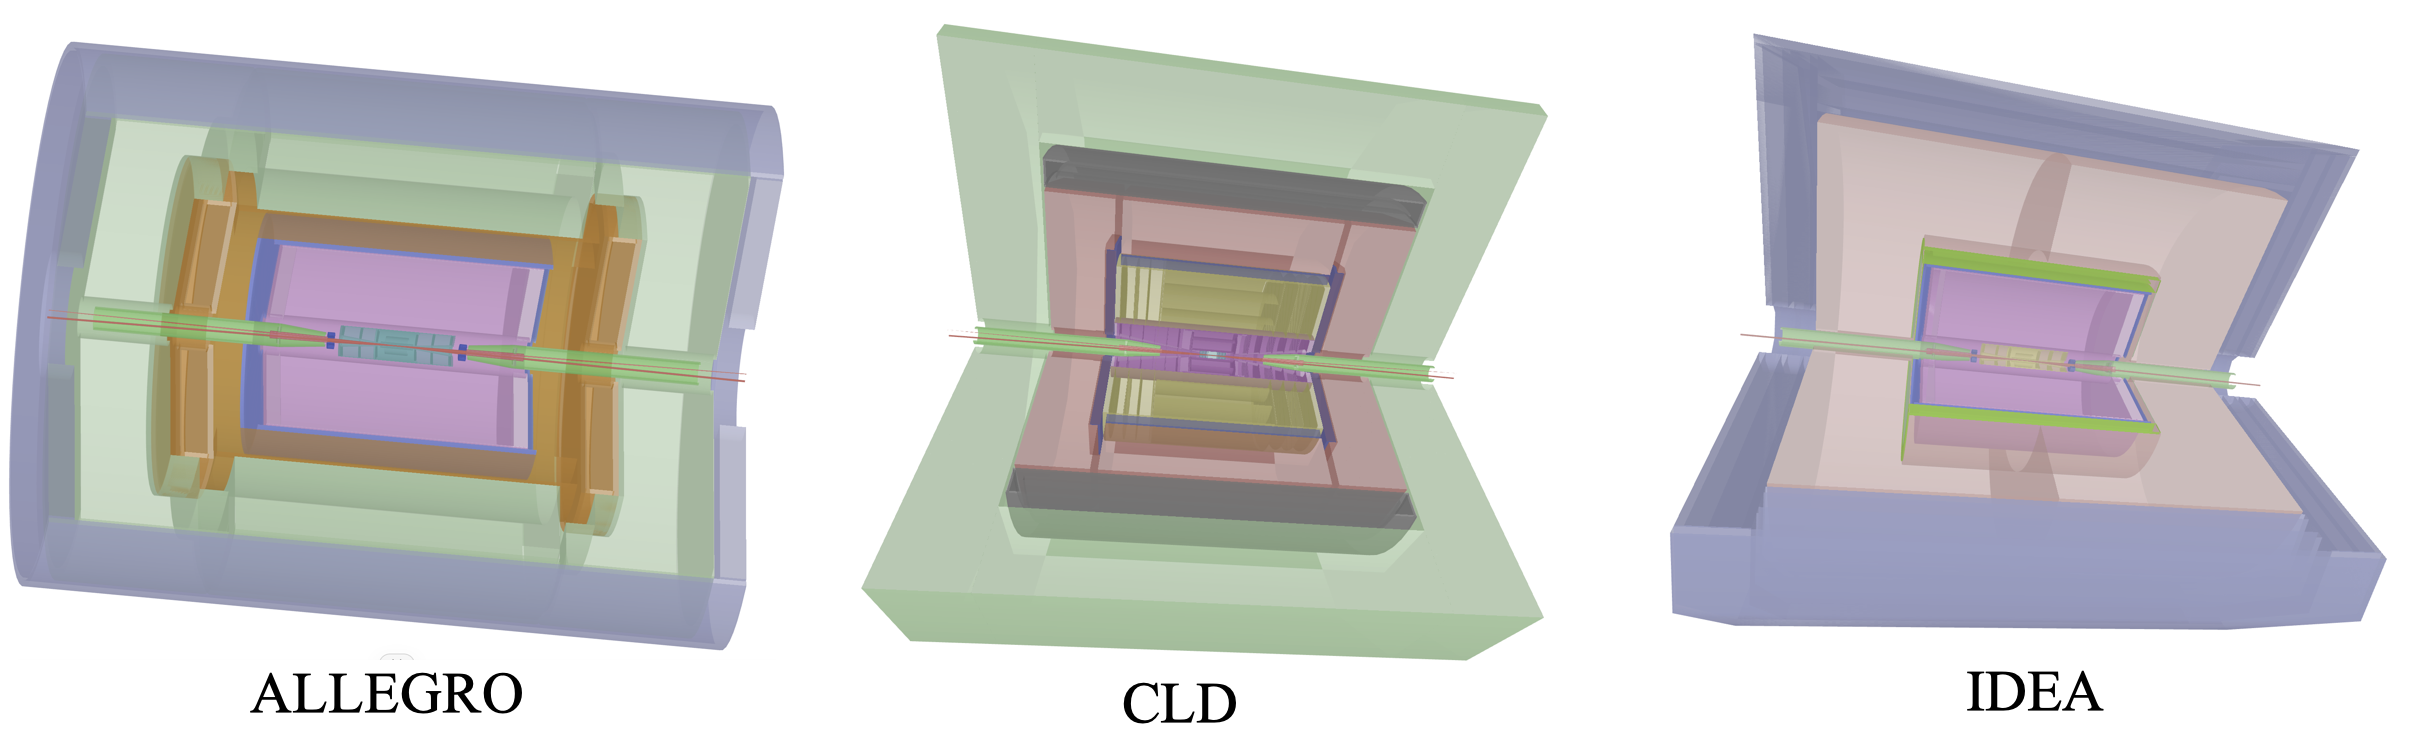
\includegraphics[scale=0.3]{Physics/SoftwareAndComputing/Figs/three_detectors_phoenix.png}
\caption{Pictures of three detector concepts (ALLEGRO, CLD, and IDEA) 
implemented in \textsc{dd4hep}.}
\label{fig:threeDets}
\end{figure}


A complete model of the CLD detector is available~\cite{CLD}. The main change with respect to the original geometry is the adaptation of the vertex detector to the most recent beam-pipe design (Section~\ref{sec:mdi}). Based on this model, an alternative option including a dedicated PID detector, named ARC, was prepared. This version of CLD features a reduced-size outer tracker in order to fit the ARC between the main tracker and the (unchanged) ECAL, as shown in Fig.~\ref{fig:CLD_ARC}. This enables comprehensive studies to evaluate the benefits of enhanced particle identification capabilities, as well as any potential impact on the performance of the particle-flow reconstruction.

\begin{figure}[ht]
\centering
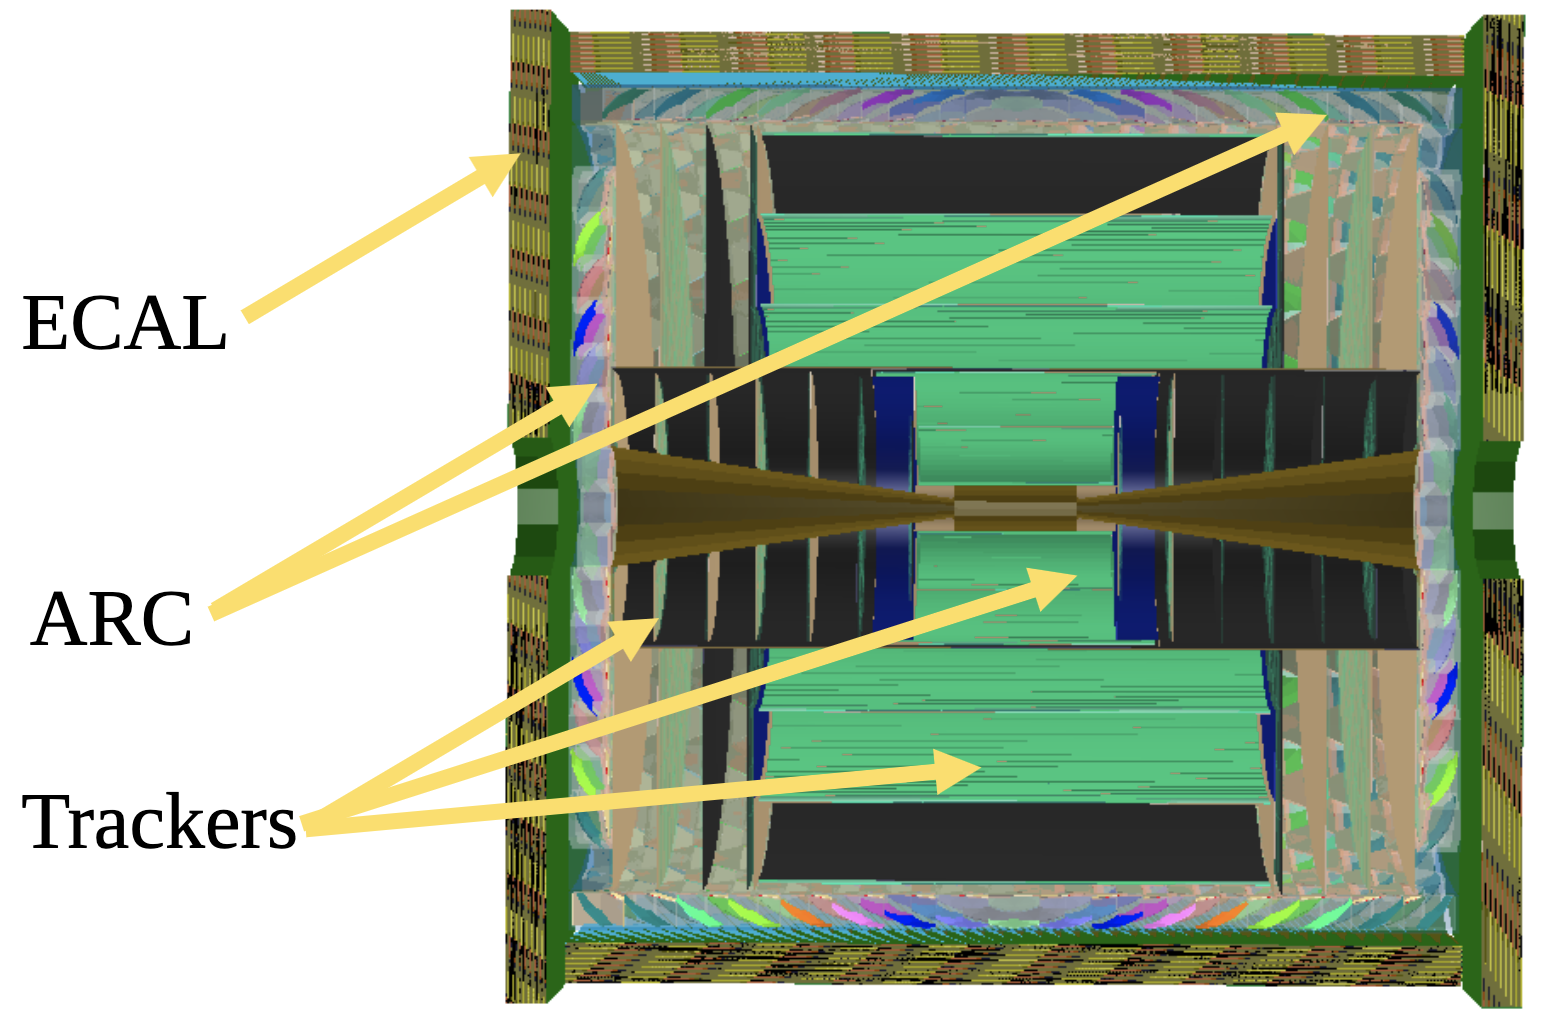
\includegraphics[scale=0.3]{Physics/SoftwareAndComputing/Figs/CLD_withARC.png}
\caption{Picture of the CLD detector concept model with enhanced particle identification capabilities. 
This variant of CLD includes the ARC sub-detector between the outer tracker and the ECAL. 
The other subsystems (HCAL, muon chambers, etc.) are present in the model but not shown here.}
\label{fig:CLD_ARC}
\end{figure}

A first complete model of the IDEA detector is also available. It consists of a detailed inner vertex detector with straight staves; a full stereo drift chamber with all wires included; a silicon wrapper constructed with the same driver as that used for the inner vertex detector;\footnote{With the options of changing the definition of the staves in the compact file to have sensitive components on both sides, using strips instead of pixels, and a reduction in the level of details being modelled to reach a computationally affordable description.} a solenoid and an end-plate absorber described as simple cylinders with a thickness $0.75\% X_0$; a pre-sampler; a fibre-based `monolithic' dual-readout calorimeter; and a $\mu$RWELL-based muon system. Based on this implementation, an alternative version of the IDEA detector, featuring an additional crystal-based ECAL, is now being developed.

The ALLEGRO detector concept is implemented as follows: a tracking system (inner vertex detector, drift chamber, and silicon wrapper) directly imported from the IDEA implementation; a noble liquid ECAL inside a lightweight cryostat whose outer wall also accounts for the solenoid material budget;  and a tile HCAL, placed inside a muon system place-holder made of two nested layers of sensitive cylinders.

The \textsc{Geant4} toolkit is used to simulate the passage of particles through matter. 
Its raw simulation output requires further processing to create data objects suitable for analysis. 
The processing workflow includes two key stages: 
digitisation, which transforms simulated detector hits into realistic detector responses, 
and reconstruction, which interprets these responses to identify and characterise the underlying physics objects. 
The next two sections provide an overview of the capabilities currently available in the central FCC software,
with ongoing developments and future directions. 
A more detailed discussion can be found in Ref.~\cite{softwareNote}.

\subsection{Digitisation} 
\label{sec:digi}

For silicon trackers and muon systems, a straightforward and generic digitisation approach is currently implemented. 
The simulated hit positions and time are smeared with Gaussian uncertainties, 
keeping the digitised hit position within the sensitive volume and applying an optional time window cut. 
The spatial smearing is performed in the local coordinate system of the sensitive module and allows for two distinct Gaussian widths. 
For strip-based sensors, the position along the strip direction is set in the middle of the sensor 
and the related uncertainty is defined as the wafer length divided by $\sqrt{12}$. 
This simple method allows a flexible and generic software implementation, making it applicable to various sub-detector types. 
An enhanced digitisation model that includes, in particular, charge-sharing effects, is under development. 
This new model will enable more detailed studies and simulations.

The digitisation of the drift chamber sub-detector follows a similar methodology. 
In this case, the two variables subject to Gaussian smearing are the distance from the simulated hit to the nearest wire 
and the position along the wire. 
In addition to producing digitised hits with smeared positions, 
the algorithm calculates the associated number of interactions (clusters) and the number of electrons emitted per interaction. 
This calculation is based on a parametrised model using the \textsc{Garfield++} simulation framework~\cite{clustercount}. 
A more detailed drift chamber digitisation, which will include the generation and analysis of full waveforms, is under development. 
This evolution will enable more reliable assessments of, e.g., the impact of beam-induced backgrounds on the drift chamber occupancy and on track reconstruction efficiency and purity.

A different approach is required for calorimeters: 
the simulated energy deposits corresponding to the same readout cell are aggregated
and a calibration factor (sampling fraction) is applied alongside other specific processes, as outlined below. 
\begin{itemize}
\item The digitisation of CLD calorimeters is based on the original \textsc{ILCSoft} implementation, interfaced with \textsc{Gaudi} wrappers and data format converters to \textsc{edm4hep}. This implementation supports per-layer sampling fractions, operates in both analogue and digital modes,
and includes zero-suppression emulation.

\item The ALLEGRO calorimeter digitiser is a ‘\textsc{Key4hep}-native’ solution 
(i.e., a \textsc{Gaudi} algorithm with \textsc{edm4hep} input and an output that does not require wrappers or converters) 
that handles radial-layer-dependent calibration, zero suppression, noise addition, and cross-talk emulation. 
The cross-talk emulation is performed in two steps: 
(1)~the derivation of a detector-specific map that encodes which cells ‘communicate’ with each other 
and the associated cross-talk coefficients (sourced from measurements for the ALLEGRO ECAL);
(2)~the detector-agnostic energy distribution across cells, following the guidelines set by the map.

\item The fibre dual-readout calorimeter digitiser accurately emulates the response of the silicon photomultiplier,
generating full waveforms based on photon arrival times using the \textsc{SimSiPM}~\cite{simsipm} package. 
This digitisation depends on parameters that can be obtained from vendors’ data sheets and accounts for a variety of effects, 
including wavelength-dependent efficiency, dark counts, after-pulsing, and cross-talk.

\end{itemize}

\subsection{Reconstruction}
\label{sec:reco}

The \textsc{edm4hep} digitised objects produced by the algorithms mentioned in the previous section 
are subsequently processed through various reconstruction routines. 
Two tracking solutions are currently used in the FCC software: 
one based on a conformal tracking implementation from \textsc{ILCSoft}~\cite{conformaltracking}, 
suitable for silicon tracking systems, 
and another based on a graph neural network~\cite{MLTRACKING_NOTE}, 
successfully applied to both silicon and gaseous trackers, 
as detailed in Sections~\ref{sec:PhysPerf_FullSim} and~\ref{sec:PhysPerf_TrackAngles}. 
The graph neural network solution currently covers only track finding;
ongoing developments will extend its capabilities to track fitting. 
Other `classical' approaches are also investigated, both for gaseous and silicon-based tracking systems.

Calorimeter clustering can be performed using three different \textsc{Key4hep}-native solutions: 
one based on a fixed-size sliding window for finding local maxima, 
another based on ATLAS topological clustering~\cite{topoclustering}, 
and the third using the CMS \textsc{clue} algorithm, 
which has been ported to \textsc{Key4hep} in the \textsc{k4clue} package~\cite{k4clue}. 
A fourth option for calorimeter clustering, used by the CLD detector, 
is available through the particle flow algorithm described below.

A particle-flow-based global event reconstruction is available in the \textsc{PandoraSDK}~\cite{pandorasdk} framework, 
which is integrated into \textsc{ILCSoft} and accessible in \textsc{Key4hep} via wrappers and converters. 
A complete particle-flow-algorithm sequence is in place for the CLD detector, adapted from the ILD solution~\cite{pandorapfa}. 
While this implementation already demonstrates excellent performance~\cite{CLD}, further optimisation is underway. 
The particle flow approach is expected to deliver the highest performance, in particular for jet energy and angular resolutions, 
making it the preferred tool for detector optimisation. 
Consequently, dedicated efforts are focused on several key areas:
\begin{itemize}
\item re-implementing the interface to \textsc{PandoraSDK} as a \textsc{Gaudi} algorithm with \textsc{edm4hep} input and output, 
eliminating the reliance on data converters and wrappers;
\item developing \textsc{PandoraSDK} sequences for the ALLEGRO and IDEA detectors, 
adapted to and exploiting the specificities of their trackers and calorimeters;
\item implementing machine learning-based particle flow algorithms using graph neural networks, 
as described in Ref.~\cite{MLPF_NOTE}.
\end{itemize}

The clustering of \textsc{edm4hep::ReconstructedParticleCollection} particle-flow particle candidates into jets 
is managed through a standard interface to the \textsc{FastJet}~\cite{fastjet} package. 
An additional \textsc{FastJet}-based interface is available for the clustering of calorimeter-only objects 
and can be used for detector setups that do not yet provide reconstructed particle candidates.

Several particle identification algorithms are, or will be, developed to further extend particle-flow capabilities with additional particle identification algorithms. 
These algorithms include a RICH pattern recognition~\cite{Forty1998} for the ARC detector (Section~\ref{sec:ARC}), 
a cluster-counting technique for gaseous trackers with d$N$/d$x$ measurement (Section~\ref{sec:Detectors_MainTracking}), 
and a jet flavour tagging using the deep-learning-based ParticleNet~\cite{particlenet} model. 
The latter is already implemented within the analysis framework described in the next section 
and is being migrated to a \textsc{Gaudi} algorithm for integration into the central reconstruction chain.

\subsection{Analysis tools}
\label{sec:analyses}

To maximise synergies and enhance the productivity of the FCC particle physicist teams, the analysis tools are centrally developed and maintained in \textsc{Key4hep}. 
The samples generated for FCC studies are stored using the \textsc{Root}-based \textsc{edm4hep} data model, 
both for the parametrised and full simulation workflows. 
Since this data model is built with the \textsc{Podio} library, 
\textsc{edm4hep} files can be analysed using the automatically generated helper methods (Section~\ref{sec:edm4hep}) 
in C++ or through the associated \textsc{Python} bindings. 
Although this is not the intended usage, those files can also be processed using `plain' (\textsc{Py})\textsc{Root}, 
i.e., without going through the \textsc{Podio} layer. 
A third solution, relying on \textsc{RDataFrames}~\cite{rdataframe}, is available through \textsc{Key4hep}. 
This package, called \textsc{FCCAnalyses}, has been central to most of the physics analyses presented in this report and is described below.

The \textsc{FCCAnalyses} package equips analysers with a comprehensive and efficient toolkit built around \textsc{RDataFrame}. 
By leveraging the \textsc{RDataFrame} framework, it provides automatic multi-threading, 
with object relations from \textsc{edm4hep} maintained in a structured tabular format 
through an \textsc{RDataSource} instance implemented in \textsc{Podio}. 
Event selection and high-level computations follow the standard \textsc{RDataFrame} syntax, 
while \textsc{FCCAnalyses} includes a set of general-purpose functions for added convenience. 
Samples and their metadata (cross sections, event counts, normalisation factors, etc.) are managed via \textsc{json} files, 
with centrally-produced samples browsable through a web interface~\cite{samplesWebPage} and available on \textsc{eos}. 
A plotting utility facilitates process normalisation, stacked histograms, and background vs.\ signal comparisons. 
In \textsc{FCCAnalyses}, histograms can be produced directly from input samples in a single step, but a `staged' workflow, 
allowing resource-intensive steps to be isolated for efficiency, is also supported. 
To enhance analysis capabilities, \textsc{FCCAnalyses} provides additional features, including the following ones.

\begin{itemize}
\item \textbf{Job submission} through \textsc{HTCondor}~\cite{htcondor} to CERN batch system.
\item \textbf{Jet clustering} via \textsc{FastJet}~\cite{fastjet} and functionalities to perform jet-parton matching.
\item \textbf{Machine learning integration} using \textsc{onnx~\cite{onnx}}, \textsc{tmva}~\cite{tmva} or \textsc{XGBoost}~\cite{xgboost}.
\item \textbf{Flavour tagging} with the deep-learning based \textsc{ParticleNet}~\cite{particlenet} model.
\item Automated \textbf{yield table production} for arbitrary cut-flows. 
\item Direct creation of \textsc{Root} files and associated data cards 
in a format suitable for the \textsc{Combine}~\cite{combine} \textbf{statistical analysis and combination tool}.
\item \textbf{Smearing tools} to generate new object collections from existing \textsc{Delphes} samples 
under different detector performance assumptions.
\end{itemize}
A more detailed overview is given in Ref.~\cite{softwareNote}.

In addition to this well-established toolkit, new initiatives aim at expanding the technology options offered to the analysers. 
For instance, the \textsc{Coffea}~\cite{coffea} \textsc{Python}-based framework, 
known for scalable, efficient processing of large HEP datasets, now supports \textsc{edm4hep}. 
The FCC software team is also exploring future-proof solutions, 
acknowledging shifts in paradigms akin to the HEP community’s transition from Fortran to C++. 
In this regard, the Julia~\cite{Julia} language, celebrated for its speed, ease of use, and expressive syntax, 
could address the `two-language problem' 
(i.e., the reliance on C++ for performance-intensive tasks and Python for user interface). 
To test Julia's suitability, an \textsc{edm4hep} format reader was developed as part of the \textsc{JuliaHEP}~\cite{juliahep} project, 
which aims to consolidate Julia-based tools for HEP.

\subsection{Visualisation}
\label{sec:visualisation}

Visual renderings of the software processes and outputs are crucial for purposes 
such as debugging, validation, physics interpretation, and outreach. 
A variety of related tools have been developed or integrated into the FCC software ecosystem, as described below.

To enable visualisation of FCC events and detectors, 
an experiment-independent web-based event display tool, Phoenix~\cite{phoenix}, 
was extended to support the \textsc{edm4hep} data model. 
Leveraging this technology, a dedicated web interface, \textsc{Phoenix@FCC}~\cite{phoenixatfcc}, 
was created to host the central versions of FCC detector geometries. 
This interface allows users to overlay event data onto a 3D view of the detector, 
with the flexibility to easily incorporate custom detectors. 
An example of an event display generated with this tool is shown in Fig.~\ref{fig:phoenix}.

\begin{figure}[ht]
\centering
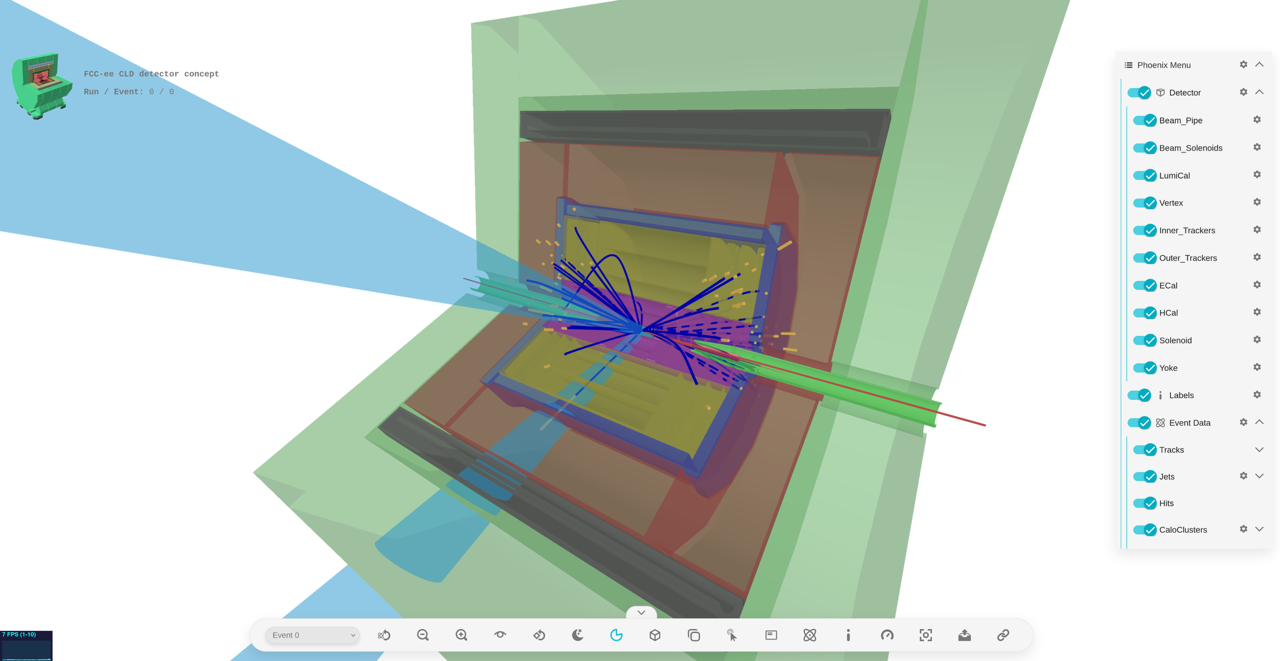
\includegraphics[width=0.9\textwidth]{Physics/SoftwareAndComputing/Figs/phoenix.png}
\caption{Visualisation of a $\ttbar$ event within the CLD detector, 
displayed using the \textsc{Phoenix@FCC} web-based event display.}
\label{fig:phoenix}
\end{figure}

Beyond the FCC-specific implementation, several other tools are available for displaying detector geometries and event content. 
These include the \textsc{JSRoot} web interface~\cite{jsroot}, 
the \textsc{Qt} plugin integrated with \textsc{Geant4} (accessible through \textsc{ddsim}), 
and the \textsc{CED} event display from \textsc{ILCSoft}~\cite{ced}.

Another visualisation tool was developed as part of the FCC studies, 
to render the content and relationships between objects in \textsc{edm4hep}-based events. 
This tool, called the \textsc{edm4hep} Event Data Explorer (\textsc{eede})~\cite{eede}, 
visualises \textsc{edm4hep} objects as boxes that display the values of their various fields and are connected to related objects 
(e.g., a calorimeter cluster will be linked to its associated individual cells). 
The displayed content can be tuned by applying filters on the objects. 
Figure~\ref{fig:eede} shows a screenshot of this tool in use, with an excerpt of a Monte Carlo generator particle tree.

\begin{figure}[ht]
\centering
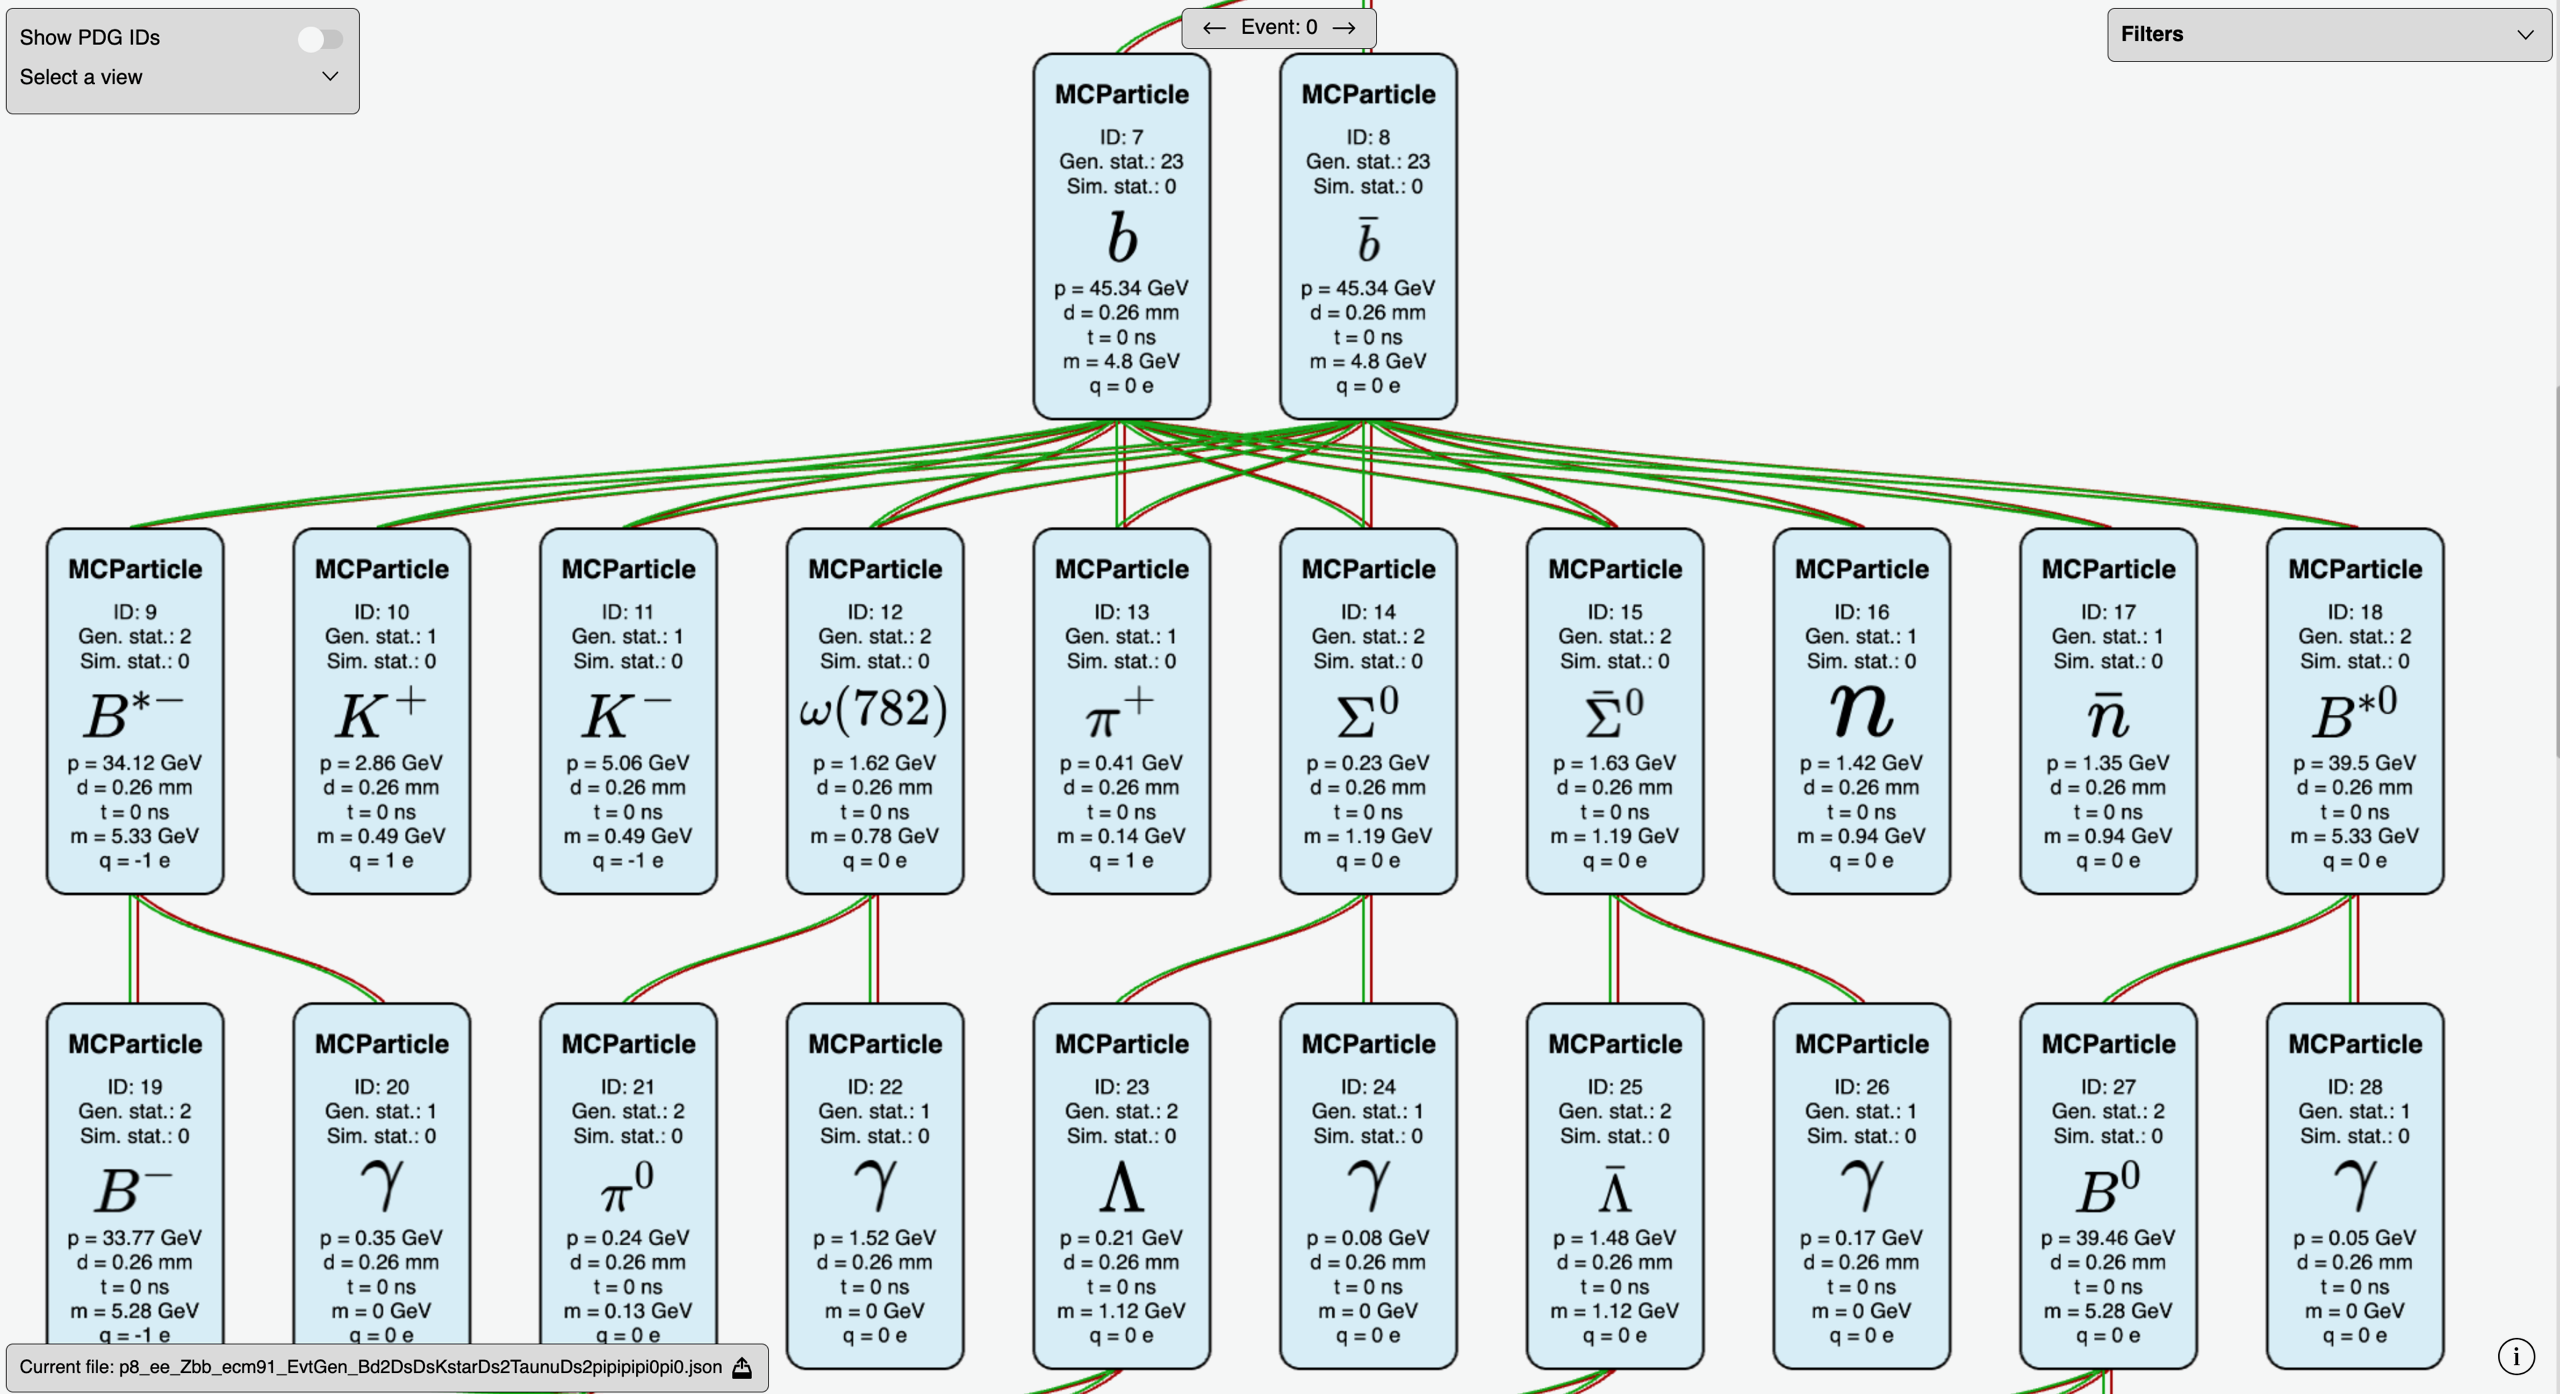
\includegraphics[width=0.8\textwidth]{Physics/SoftwareAndComputing/Figs/eede_Zbb_hadronisation.png}
\caption{Visualisation of the Monte Carlo particle tree for an $\epem \to \PZ \to \PQb\PAQb$ event,
generated using the \textsc{edm4hep} Event Data Explorer~\cite{eede}.}
\label{fig:eede}
\end{figure}

\subsection{Computing resources}
\label{sec:resource}

The computing resource requirements of a project include the processing power necessary to manage the data generated by its activities 
and the storage capacity needed to maintain those data samples at various stages of processing. 
During the Feasibility Study, the work of particle physicists has primarily focused on `offline' activities, 
which correspond to the workflows in Fig.~\ref{fig:workflows}. 
These activities are expected to remain central during the next phase of the study.
An initial analysis of the FCC offline computing needs is presented in Ref.~\cite{ganhelfccres}. 
This section builds upon and expands that analysis, with further insights. 

The FCC PED activities to date have primarily relied on resources provided by CERN, as displayed in Table~\ref{tab:cernres}. 
These resources represent approximately 0.1\% of those currently available to the LHC experiments, and will need to substantially increase.
The main purpose of this section is to give enough elements to provide reasonable projections of the needs, 
as a function of parameters that will be better defined as the project progresses. 
Current ideas to ensure that an adequate amount of resources is available for the studies are also presented.
The target timescale is that of the next phase of the study (2025--2027), 
possibly extending to the first years of the proto-collaboration forming phase (2028--2030). 
A projection to the needs of the actual \PZ-pole operations, in two decades from now, is also presented.

\begin{table}[t]
\centering
\caption{Resources available at CERN for FCC physics, experiments and detectors studies as of October 2024. 
The (old) benchmark HepSpec06 (HS06) is still used to facilitate comparison with LHC numbers; 
for the purpose of this analysis, HS06 and HS23 are numerically equivalent.}
\label{tab:cernres}
\begin{tabular}{c l}
\toprule
\multicolumn{2}{c}{Storage on \textsc{eos}} \\
\midrule
600\,TB & for central productions \\
100\,TB & for analysis \\ 
\midrule
\multicolumn{2}{c}{Processing power} \\ 
\midrule
9000 HS06 / HS23 & CPU on lxbatch \\
3 GPU & nodes on CERN Openstack \\
Some GPU & nodes on EuroHPC (via CERN OpenLab) \\ 
\bottomrule
\end{tabular}
\end{table}

\subsubsection{Resource modelling} 
\label{sec:resourceshllhc}

Reliable projections require a model for the resource needs. 
When discussing the computing resource needs, it is necessary to treat the two main phases of the project separately: 
design and preparation on the one hand, and data taking on the other.
During the design and preparation phase, the studies are performed with simulated and test-beam data, with needs increasing with time, based on expected integrated luminosities that define the statistical framework, and with many moving targets and unstructured activities (such as the number and type of detector concepts, data formats, algorithms, and levels of software optimisation). During the collider operation, both collected and simulated data need to be processed continuously, with more stable versions of detector implementations, data formats, and core-software, 
albeit with quasi-stable algorithms that will continue to be refined during the operations phase. 

The significant and sustained effort dedicated to modelling the computing resource needs in ATLAS and CMS has been thoroughly documented, and has quantified both the short- and long-term projections for the high-luminosity LHC programme. An example can be found in Ref.~\cite{langecmsres}. The most recent update is shown in Fig.~\ref{fig:resourceshllhc}, from the latest CMS~\cite{CMSreshllhc} and ATLAS~\cite{ATLASreshllhc} approved figures, with similar real and simulated data samples. Not surprisingly, the projected needs are shown to decrease with more aggressive R\&D efforts. In particular, past investments in R\&D, software quality/performance improvement, and optimal use of storage in the past decade, have proven to be critical in reducing the HL-LHC computing needs of the experiments. The projected needs are compared to the extrapolated available computing capacities under a sustainable flat budget model. 
From theses numbers, it is possible to derive that both ATLAS and CMS will have storage needs of the order of a few EB and computing needs of the order of a few MHS06.\footnote{An HS06 = HEPSpec06 is a benchmark to measure the computing capacity of a Computing Element. 
The rule of thumb `core = 10 HS06' is used for the hardware available (at the time of writing) at, for example, the CERN facilities.}

\begin{figure}[ht]
\centering
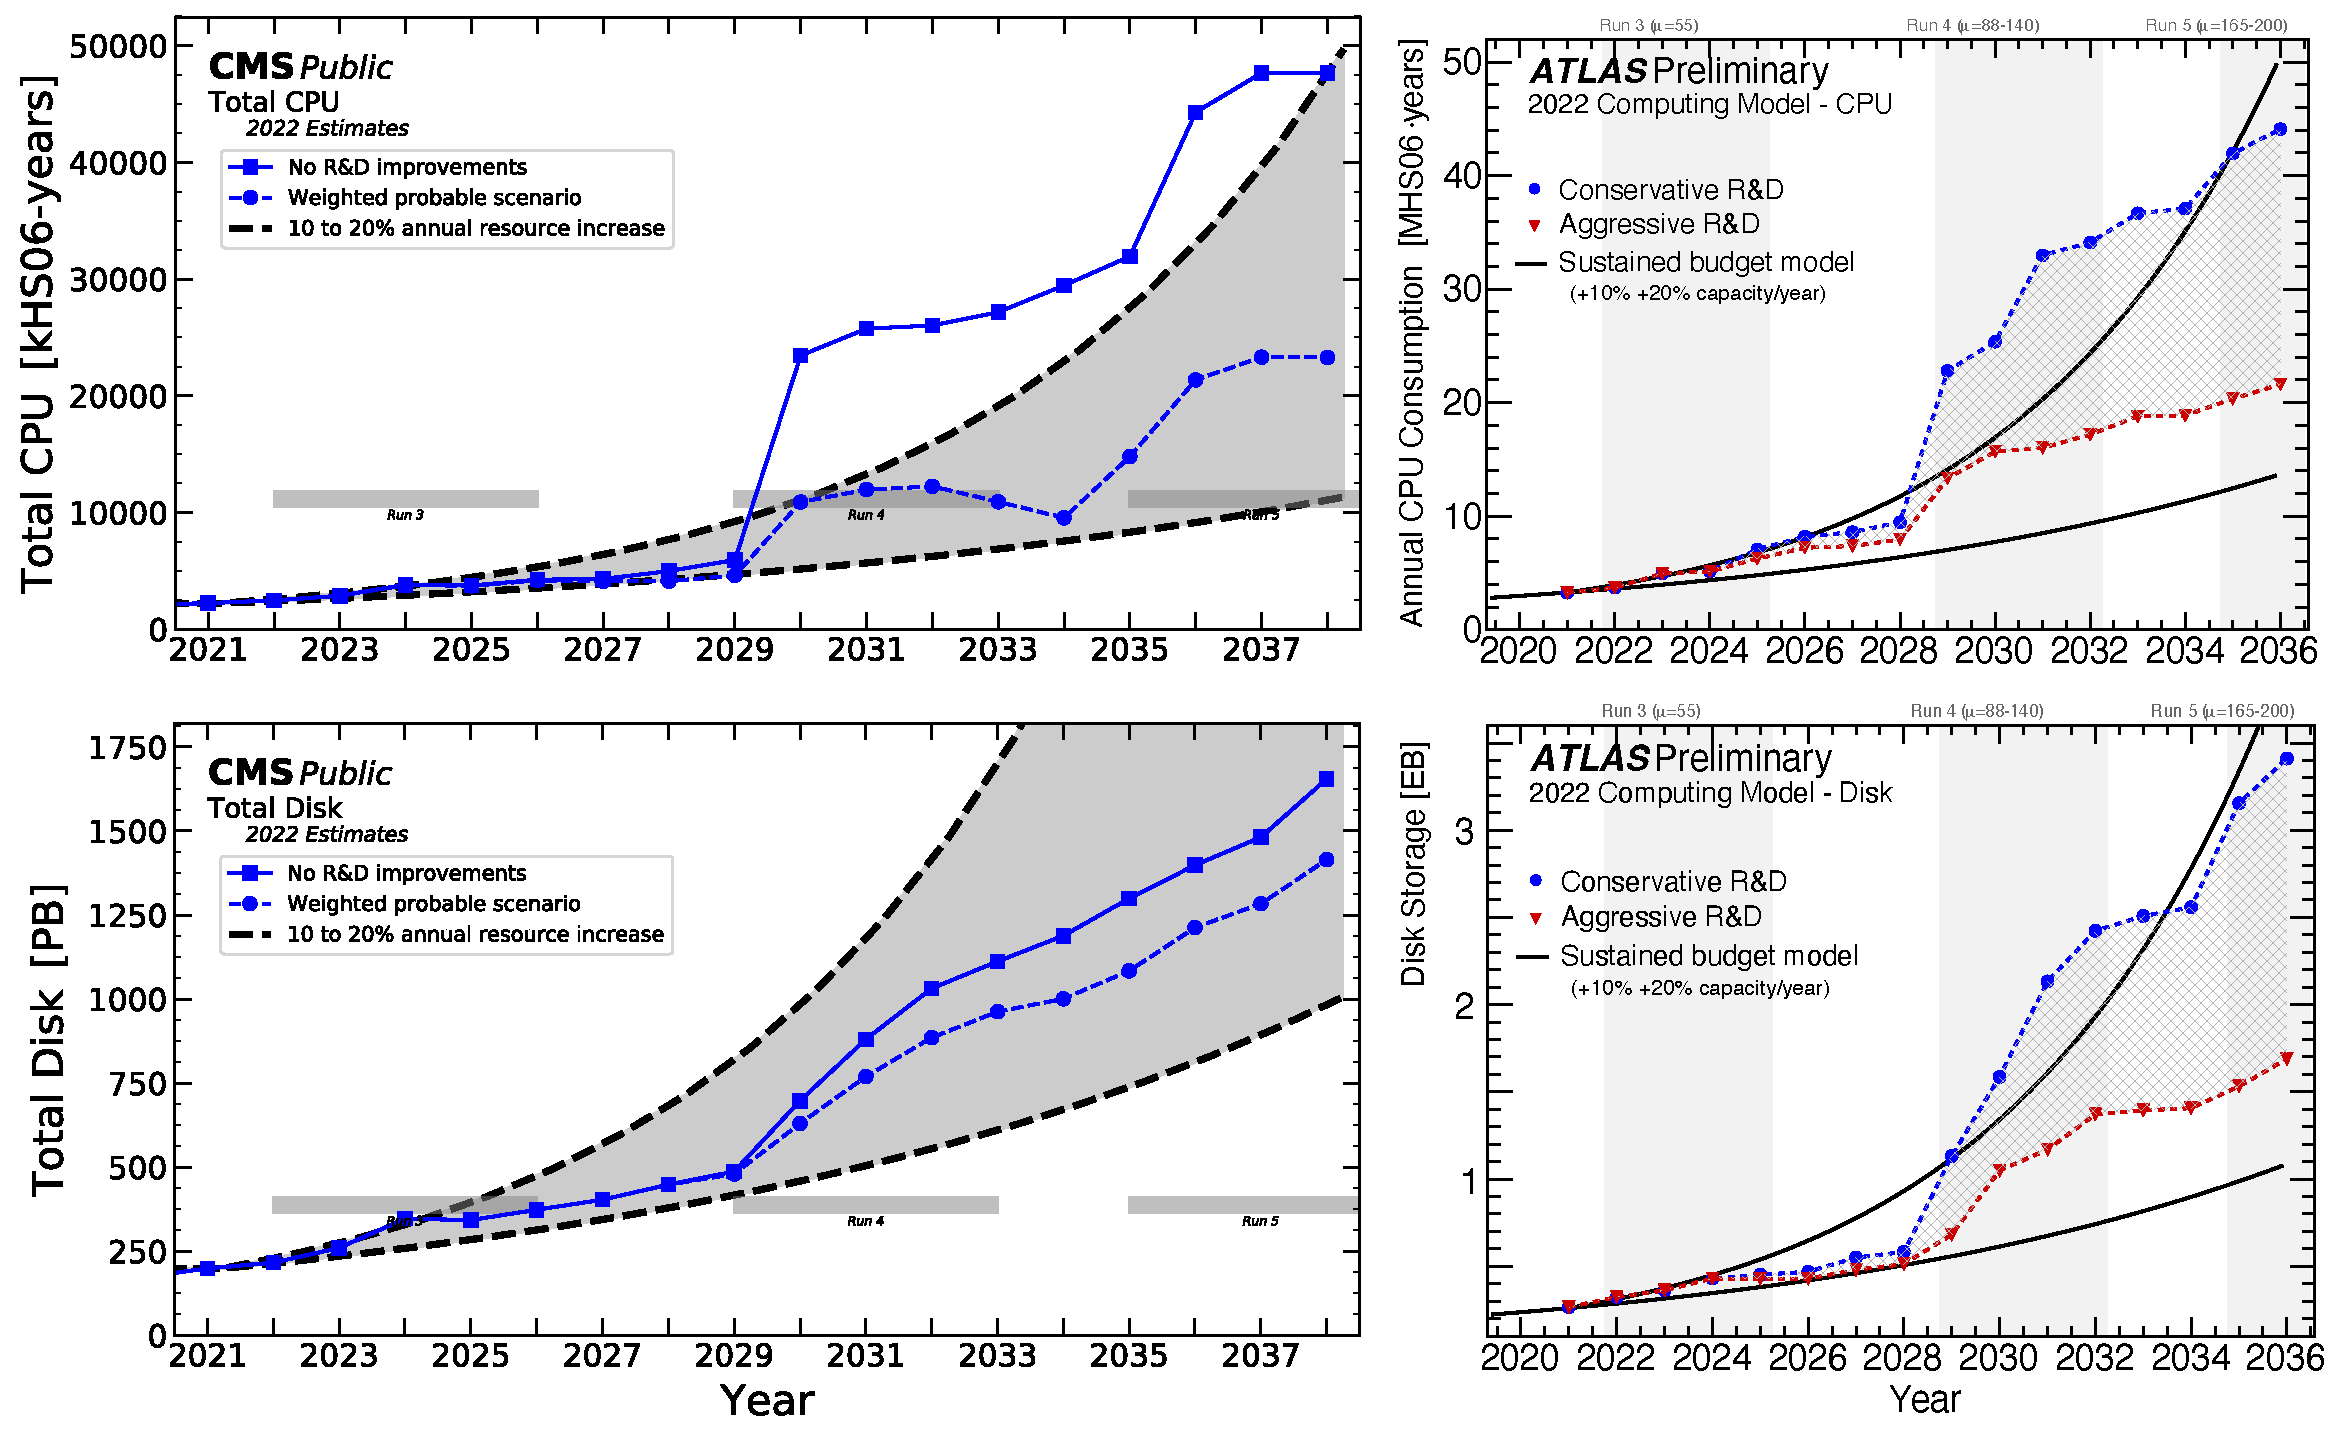
\includegraphics[width=\textwidth]{Physics/SoftwareAndComputing/Figs/ATLAS-and-CMS-HL-LHC-projections.pdf}
\caption{Projections of CMS (left) and ATLAS (right) computing (top) and storage (bottom) resource needs for HL-LHC. 
In both cases, the demands in case of no or conservative R\&D and planned or aggressive R\&D 
are compared with projections of future pledged resources. 
From Refs.~\cite{CMSreshllhc} and~\cite{ATLASreshllhc}. 
For ATLAS and CMS, the data and Monte Carlo samples have roughly the same size~\cite{PiparoPriv}.}
\label{fig:resourceshllhc}
\end{figure}

The basic concepts of resource modelling employed by the LHC experiments can be applied to the FCC case, which 
boils down to identifying the activities and the corresponding set of objectives and required workflows. 
The detailed activities and objectives depend on the phase of the project, although macro-activities can be present at all stages.
Today, and in the near future, the identified macro-activities include data analysis, sub-detector development and optimisation, and algorithm design and optimisation.

\paragraph{Data analysis}

This activity will always be present, in all phases of the project. 
During the design phase, the goal is to study the potential of the project with a level of accuracy that depends on the aspect being investigated. 
A first feasibility study of a measurement is typically done using a parametrised simulation of the response of a given detector concept, 
to identify critical points that would require a more accurate simulation. 
Parametrised (or fast) simulation is also required for an experiment during data taking, e.g., for a rapid exploration of large portions of parameter space. 
As the studies progress, the need for accuracy increases, which calls for  fully-simulated and properly-reconstructed events. 
Therefore, the analysis activity will always bring requirements for adequate samples of parametrised and fully simulated-reconstructed events, 
their relative importance depending on the phase of the project. 
An example of a presently ongoing analysis macro-activity with full simulation is discussed in Section~\ref{sec:PhysPerf_FullSim}. 

\paragraph{Sub-detector development and optimisation}

This activity is specific to the design phase, during which the detector response is simulated,
primarily using particle guns to generate particles of a specific type, within a given region of phase space. 
Additionally, samples of simulated events may prove useful and serve as benchmarks for the design process.
While the size of these samples is usually not enormous, 
they may require a higher level of detail than is typical for standard physics analyses, 
potentially resulting in large data volumes. 
Examples of such activities are discussed in Chapter~\ref{sec:concepts}.

\paragraph{Algorithm design and optimisation}

This activity is present during all phases of a project. 
During the design phase, a minimal set of algorithms is identified to evaluate the performance of the proposed (sub)detectors, and to subsequently improve and tune their design. 
During later stages, when the detector design is frozen (or when the detector is built), the algorithms are continuously developed for improved performance. 
This activity makes use, in particular, of particle guns and simulated events enriched in certain topologies. 
Examples of such activities are presented in Chapter~\ref{sec:requirements}.
Advanced AI approaches, such as ML-based tracking and particle flow algorithms, are complementary to more classical approaches in both the design and production phases. During the design phase, they offer a rapid re-optimisation of varying designs and concepts; during the production phase, they are expected to deliver better performance.

\subsubsection{Modelling resources for FCC-ee}

At this stage, quantitative predictions are only possible for the analysis macro-activity. The necessary basic ingredients are the event sizes and the event processing time. The current activities mostly use parametrised simulations, hereafter labelled \textsc{Delphes}, 
for which rather complete sets of events have been produced. 
The numbers presented in the following are taken from the \emph{Winter 2023} production campaign. 
For the full simulation, some measurements have been performed with the simulation of selected samples with CLD, taken as a reference. 
It is assumed that the event sizes and the event processing times scale in the same way as for \textsc{Delphes}. 
This assumption is based on the fact that these numbers depend mostly on the number and type of particles, 
and that they affect the sizes and processing time in the same way in \textsc{Delphes} and full simulation.
The resulting event sizes and processing times are reported in Table~\ref{tab:baselinesizes}. 

\begin{table}[ht]
\centering
\caption{Baseline event sizes and processing times. Parametrised simulation and full simulation with \textsc{Geant4} are denoted  
\textsc{Delphes} and \textsc{Full}, respectively. For \textsc{Full}, the values are extrapolated from measurements performed with $\PZ \to \PQq\PAQq$ events, under the assumptions described in the text. }
\label{tab:baselinesizes}
\begin{tabular}{c c c c c c }
\toprule
Process & $\sqrt{s}$ & \multicolumn{2}{c}{Size / event } & \multicolumn{2}{c}{Processing time / event }  \\ \cline{3-6}
$\epem \to$ & (GeV) & \textsc{Delphes} (kB) & \textsc{Full} (MB) & \textsc{Delphes} (ms) & \textsc{Full} (s) \\ 
\midrule
$\PZ \to \PQq\PAQq$, $\ell^+\ell^-$ & 91.18 & 8.3, 1.2 & 1.1, 0.16      & 14, 0.5 & 11, 1.6 \\
$\PWp\PWm \to \text{all}$, $\PGn\PAGn \ell^+\ell^-$ & 157--163 & 9.5, 1.2 & 1.3, 0.16 & 16, 0.5 & 13, 1.6 \\
$\PH\PZ \to \PGn\PAGn \PQb\PAQb$, $\PQb\PAQb \PQb\PAQb$ & 240 & 8.9, 13 & 1.2, 1.8    & 15, 23 & 12, 18 \\
$\PZ\PZ \to \text{all}$ & 240 & 10 & 1.4                              & 17 & 13 \\
$\ttbar \to \text{all}$ & 365 & 18 & 2.3                           & 30 & 23 \\ 
\bottomrule
\end{tabular}
\end{table}

To project the needs in the years to come, 
an assumption on the needs in terms of sizes of the simulated samples has been made. 
A rule of thumb often used to get approximate values is to assume simulated samples corresponding to the expected integrated luminosity at each centre-of-mass energy, 
as displayed in Table~\ref{tab:seqbaseline} of this report. 
Table~\ref{tab:baselineneedsfull} shows the corresponding needs, for one experiment, in terms of computing resources.

Reconstruction and analysis requirements are not included in Table~\ref{tab:baselineneedsfull} 
because of the lack of sufficient quantitative information. 
However, the size of the \textsc{Delphes} output, designed to emulate the reconstruction process, 
can serve as a basis for estimating the reconstruction needs. 
While the actual reconstruction may require more detailed information than what is currently provided by \textsc{Delphes}, 
it is unlikely to significantly impact the overall resource demands. 
This conclusion is even clearer for the final analysis ntuples, which represent a condensed version of the \textsc{Delphes} output.
The processing power needs are more difficult to quantify. 
For reference, at LEP and Belle~II, the reconstruction step took about 30\% of the full simulation CPU time~\cite{ganhelfccres}, 
which can be taken as a conservative estimate, given that (opportunistic) heterogeneous resources can play a relevant role in here.
The numbers reported \emph{for one experimennt} in Table~\ref{tab:baselineneedsfull} 
give therefore a reasonable estimate of the scale of the 
problem.\footnote{It should be noted that, for \textsc{Delphes}, 
in principle the sample can be reused for a different \emph{detector concept} on the fly 
with minimal use of additional processing resources.}
These numbers show that the computing needs for the \PZ run are of the same order of magnitude as those 
of ATLAS and CMS  for HL-LHC. For the other runs, instead, the table shows that full nominal integrated luminosity samples are achievable today.

\begin{table}[t]
\centering
\caption{Projected needs for the nominal integrated luminosity, for one experiment. 
The amount of HS06 is shown for a reference period of three years, i.e., roughly the duration of the next phase of the study.}
\label{tab:baselineneedsfull}
\begin{tabular}{c c c c c c c}
\toprule
    &         &  & \multicolumn{2}{c}{\textsc{Delphes}}  & \multicolumn{2}{c}{\textsc{Full}} \\ \cline{4-7} 
\multirow{2}{*}{Run} & \multirow{2}{*}{Process} &   Number & Storage & CPU & Storage & CPU \\
    &         &   of events & (PB)          & (HS06) & (PB)        & (HS06) \\ \midrule
\multirow{2}{*}{\PZ} & $\PQq\PAQq$     &  1500 G  & 12.5          & 2.2 k  & 1650         & 2 M \\ 
   & $\ell^+\ell^-$    &  225 G   & 0.275         & 12    &   40         & 40 k \\ \midrule
\PW & $\PWp\PWm$      &  60 M    & $\sim 10^{-3}$&       & 0.075        & 72 \\ \midrule
\multirow{2}{*}{$\PH\PZ$} & $\PH\PZ$     &  500 k   & $\sim 10^{-5}$&       & $\sim 10^{-3}$ & $\sim 1$ \\ 
   & $\rm VBF\-H$ &  16 k    & $\sim 10^{-6}$&       & $\lesssim 10^{-3}$ &  \\ \midrule
\multirow{3}{*}{top} & $\ttbar$ &  500 k   & $\sim 10^{-5}$&       & $\sim 10^{-2}$ & $\sim 1$ \\ 
   & $\hz{}$      &  90 k    & $\sim 10^{-6}$&       & $\lesssim 10^{-3}$ &  \\ 
   & VBF\,H &  23 k    & $\sim 10^{-6}$&       & $\lesssim 10^{-3}$ &  \\ \midrule
\multicolumn{2}{c}{Total} &  1725 G    & {\bf 13}           & 2.2  & {\bf 1690} & {\bf 2 M} \\ 
\bottomrule
\end{tabular}
\end{table}

\subsubsection{Minimal baseline working scenario}

These considerations enable the design of a minimal working scenario to serve as a baseline target. 
This scenario includes, as a minimum, full nominal integrated luminosity samples for the \PW, $\PH\PZ$, and $\ttbar$ datasets, 
as well as `sufficiently large' samples for the \PZ run, 
where the precise definition of `sufficiently large' remains to be determined.
Table~\ref{tab:baselineneedsplan} reports the values, assuming that `large enough' means 100 times the LEP event samples.
The total values per detector and for all four detector concepts are also provided, assuming that they have similar average demands. 
These numbers are not far from the resources currently available and are well within the range of what can be realistically achieved, 
as discussed later. 
Consequently, the baseline `100$\times$LEP' scenario appears to be a realistic and achievable target.

\begin{table}[ht]
\centering
\caption{Projected needs for one experiment, 
for the scenario with nominal integrated luminosity samples for the \PW, $\PH\PZ$ and $\ttbar$ runs, 
and event samples 100 times larger than the LEP samples for the \PZ run. 
The total corresponds to four experiments requiring the same resources. 
The amount of HS06 is shown for a reference period of three years, i.e., roughly the duration of the next phase of the study. 
The totals in bold are beyond today’s availability.}
\label{tab:baselineneedsplan}
\begin{tabular}{c c c c c c c}
\toprule
    &         &  & \multicolumn{2}{c}{\textsc{Delphes}}  & \multicolumn{2}{c}{\textsc{Full}} \\ \cline{4-7} 
\multirow{2}{*}{Run} & \multirow{2}{*}{Process} &   Number & Storage & CPU & Storage & CPU \\
    &         &   of events & (TB)          & (HS06) & (TB)        & (HS06) \\ \midrule
        \PZ & $\PQq\PAQq$    &  400 M    & 3.25        & $\sim 1$  & 440     & 475 \\ 
        (100$\times$LEP) & $\ell^+\ell^-$ &  42.5 M   & 0.05        &           & 6.5     & 7 \\ \midrule
        \PW & $\PWp\PWm$     &  60 M     & 0.6         &           & 75      & 72\\ \midrule
\multirow{2}{*}{$\PH\PZ$} & $\PH\PZ$    &  500 k     & 0.0065      &           & 1       & $\sim 1$ \\ 
                & VBF\,H &  16 k  & $\sim 0.001$ &           & 0.25    &  \\ \midrule
\multirow{3}{*}{top} & $\ttbar$ &  500 k     & 0.009       &           & 9       & $\sim 1$ \\ 
                & $\PH\PZ$     &  90 k  & $\sim 0.001$ &           & 0.2     &  \\ 
                & $\rm VBF\-H$&  23 k   & $\sim 0.001$ &           & 0.25    &  \\ \midrule
\multicolumn{2}{c}{Total}        &  500 M    & 4           & $\sim 1$  & {\bf 530} & {\bf 550} \\ 
\multicolumn{2}{c}{4 experiments}        & 2000 M    & 16          & $\sim 4$  & {\bf 2100} & {\bf 2200} \\ 
\bottomrule
\end{tabular}
\end{table}

Efficiently managing limited computing resources requires a three-fold optimisation approach for the software, the analysis techniques, and the workload and data management. A proactive approach to resource management is essential for securing ongoing support from official bodies, 
especially as computing needs continue to grow. The following paragraphs discuss the current (or planned) pertinent investigations. 

\subsubsection{Optimising resources: Software}

\paragraph{Software quality and efficiency improvements}

Upgrading the code quality and efficiency is fundamental, though it often involves a considerable investment in time and expertise. 
By continually using the latest software versions, projects can leverage optimisations and new capabilities. 
For instance, recent updates to \textsc{Geant4} have nearly doubled the speed of simulation for the ATLAS experiment, 
illustrating the potential performance gains achievable through modernised codebases. 
Moreover, new, faster simulation techniques are emerging and being integrated in the software frameworks 
for use in production\footnote{Parts of the electromagnetic calorimeter of ATLAS are simulated with Machine Learning techniques.}, 
and may offer further efficiency improvements. 
End-to-end fast simulation based on Machine Learning techniques are also being developed, 
which could provide interesting ways to test very large event samples~\cite{flashsim-chep24}. 

\paragraph{Selective and filtered simulation approaches}

Another opportunity for optimisation lies in selective or filtered simulations. 
By applying filters at the generation stage, 
simulations can focus only on event components relevant to specific analyses, 
reducing unnecessary computation. 
For example, simulating only sub-detectors relevant for a given study could save substantial processing power. 
This strategy requires a careful balance between computational savings and scientific accuracy, but could significantly improve throughput.

\paragraph{Leveraging heterogeneous resources for reconstruction and analysis}

Heterogeneous computing environments, combining CPUs, GPUs, and other accelerators, 
offer significant opportunities for resource optimisation, particularly for computationally intensive tasks such as reconstruction and analysis. 
This approach has already proven highly valuable at the LHC, where the use of GPUs and specialised hardware for suitable tasks has improved efficiency, 
freeing traditional CPU resources for other activities. 
Extensive R\&D programmes are underway to develop the potential of these technologies in view of 
HL-LHC.\footnote{An example is the Next Generation Trigger project~\cite{kickNGT}.} 
Integrating these advances into the FCC software ecosystem to ensure seamless compatibility and optimal performance 
across diverse processing architectures is of critical importance for the FCC project.  
    
\subsubsection{Optimising resources: Analysis techniques}

\paragraph{Enhanced interplay between full and parametrised simulation}

In scenarios where full simulation is unnecessary, parametrised simulations, such as those provided by \textsc{Delphes}, 
can produce sufficiently accurate results with far lower resource demands. 
Facilitating interaction between full and parametrised simulations allows researchers to switch between these approaches as needed, 
optimising resource use for each stage of an analysis. 
Developing automated or optimised configurations for \textsc{Delphes} would further support this flexibility, 
making it easier to adapt simulations based on the specific needs of each analysis.

\paragraph{Advancing beyond traditional statistical methods}

By default, HEP analyses rely on a straightforward rule of thumb: 
generating MC samples at least as large as the expected data sample. 
While simple, this approach is resource-intensive, particularly in scenarios with high data volumes and complex simulations. 
Alternative statistical methodologies that allow similar statistical power with fewer simulated events 
are already explored in some fast simulation domains with promising results~\cite{varred}; 
these variance reduction techniques should be further investigated to optimise computational resources.    

\subsubsection{Optimising resources: Workload and data management}

A home-made solution effectively supported the production on the local CERN \textsc{HTCondor} and \textsc{eos} resources until the time of writing. 
The increasing complexity and scale of FCC projects necessitate a more robust and distributed infrastructure.
The primary requirements for the updated system include: 
a centralised file catalogue to organise and track data;
data replication to ensure redundancy and accessibility across sites; 
and remote access capabilities to facilitate seamless interaction with distributed resources.

To address these FCC needs, \textsc{iLCDirac}, the instance of the \textsc{Dirac} framework used in past linear collider studies, has been adopted. 
This framework is widely recognised for its workload management and file catalogue capabilities, and is already employed by several high-energy physics experiments, such as LHCb, Belle~II, BES~III, JUNO, etc. 
Through this integration, the FCC Virtual Organisation (FCC~VO) has become part of \textsc{iLCDirac}.
The CERN \textsc{HTCondor} and \textsc{eos} resources have been associated with the FCC~VO within \textsc{iLCDirac}. 
In addition, steering applications tailored to FCC workflows have been integrated into the framework 
to support specialised production needs.

Production with \textsc{iLCDirac} has begun, marking significant progress in adopting the distributed model. 
Efforts to include external storage elements (SE) have been initiated with sites at CNAF, Bari, and Glasgow. 
While these integrations are still in the testing phase, 
they represent an essential step towards expanding the infrastructure capacity and flexibility.
This approach ensures that FCC projects benefit from a scalable and distributed workload management system, 
ready to handle the challenges of future production and analysis tasks.

\subsubsection{Increasing available resources: pledged resources}

At CERN, FCC currently obtains computing resources from quotas reserved for the `Small and Medium Experiments' (SME) projects. 
These resources, while sufficient for initial activities, are limited and cannot realistically be increased by a large factor in the SME context. 

To address future needs, 
discussions are ongoing with the WLCG and CERN resource management teams to integrate FCC into the WLCG computational infrastructure. 
This integration, which should begin as early as 2025, 
would establish a reliable framework for resource allocation and enable a steady increase in computing and storage capacity over time. 
Current projections suggest that, by the end of the next phase of the study, in 2027, 
a tenfold increase in resources should be achievable, equivalent to approximately 5\,PB of storage and 100\,kHS06 of CPU power. 
These resources would be sufficient to support the minimal baseline `100$\times$LEP' scenario discussed earlier, 
while also providing contingency for targeted studies requiring larger data samples.

\subsubsection{Increasing available resources: opportunistic resources}

To enhance resource availability for FCC projects, leveraging opportunistic resources is a key strategy, which includes high-performance computing (HPC) facilities, national resources, and advanced development initiatives.

On the HPC front, discussions are ongoing with CERN OpenLab to exploit EuroHPC resources for FCC needs. 
The focus is on providing transparent access through the CERN OpenLab interface, 
which is being developed to support diverse hardware architectures, such as AMD, Intel, and ARM CPUs, as well as NVIDIA and AMD GPUs.
Initial estimates suggest access to substantial computing resources over periods ranging from six months to one year, 
which would support specific, time-limited studies requiring intensive computational power.
Investigations are underway to integrate these HPC resources into \textsc{Dirac}, ensuring streamlined access for FCC workflows.
The HPC resources are particularly suitable for specialised use cases that demand intense but temporary computational efforts, 
such as AI and machine learning (ML) developments, and
physics-specific simulations or statistical studies requiring short-term bursts of computing power.

Resources available at individual institutes or through national departments could significantly contribute to FCC workloads. 
These resources can potentially be included within the FCC~VO through integration with the \textsc{Dirac} framework, 
enhancing the overall pool of accessible computational power.

\subsubsection{Projecting to the \texorpdfstring{\PZ}{Z} run}

All the above provides a basis for understanding the computing needs during the \PZ run. 
The analysis focuses on storage requirements, likely to be the most critical aspect.
The squares in Fig.~\ref{fig:StorageProjZRun} show the projected FCC storage requirements for the real data collected during the \PZ-pole
run,\footnote{A similar situation applies to CPU needs, 
though it is important to consider the previously mentioned challenge of adapting to heterogeneous resources. 
Nonetheless, it is anticipated that by 2045 this issue will likely no longer be a significant obstacle.} with four experiments and the assumption of four identical runs in four years. Also shown are 
the projections for simulated data with size identical to the real data (triangles), four times larger than the real data (stars) and ten times larger than the real data (circles). 
The horizontal band indicates the HL-LHC's projected storage requirements, 
as derived from Fig.~\ref{fig:resourceshllhc} assuming that ATLAS and CMS account for approximately 90\% of the total.

\begin{figure}[t]
\centering
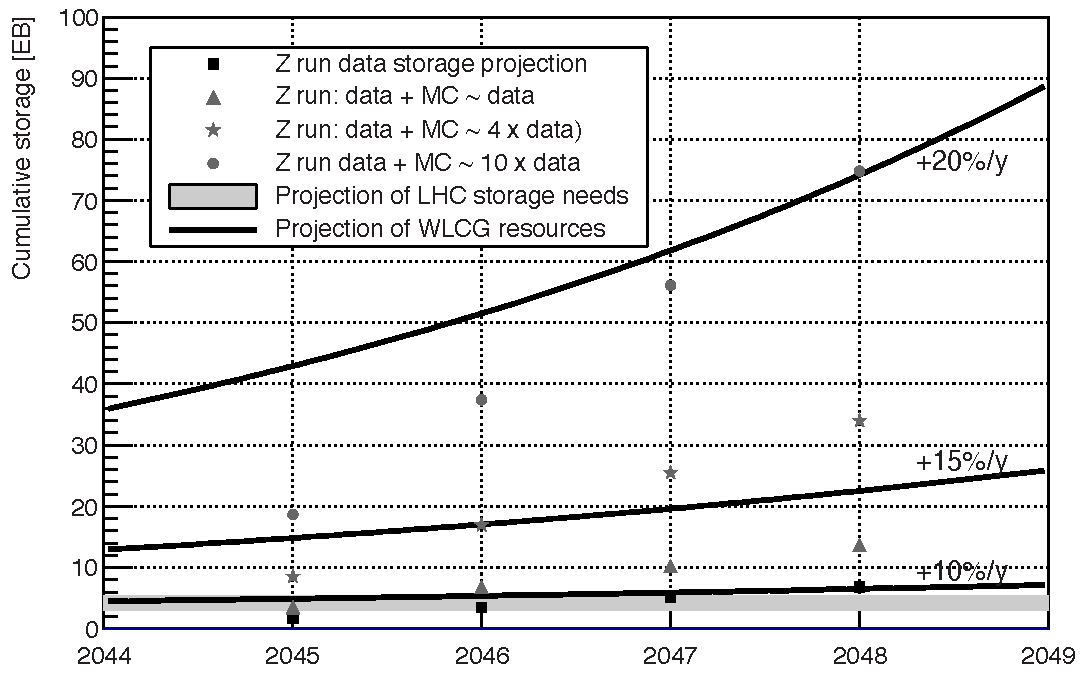
\includegraphics[scale=0.7]{Physics/SoftwareAndComputing/Figs/Storage-Projection-Zrun.pdf}
\caption{Projection of the current storage resources to the FCC-ee \PZ-pole run with four experiments collecting equal amounts of data in four successive years (squares) 
and varying amounts of simulated data (triangles, stars, circles). 
The figure also includes the projected resource needs of the LHC and a hypothetical evolution of WLCG resources, under different scenarios for sustained annual budget increases.}
\label{fig:StorageProjZRun}
\end{figure}

The storage resources required for FCC-ee data during the \PZ run are comparable to the projected requirements of the LHC. 
The inclusion of simulated samples, however, will substantially increase the storage demands, even in the minimal scenario, 
in which the simulated samples have a size similar to that of the real data samples. A dedicated computing infrastructure, 
similar to the World LHC Computing Grid (WLCG) for the LHC, is therefore required to meet the computing demands of the FCC. 
As previously mentioned, this could possibly be a natural extension of the WLCG. 
The projected storage capacity of the WLCG during the years of the FCC-ee \PZ-pole run, 
under various assumptions regarding sustained annual budget increases, is also shown in Fig.~\ref{fig:StorageProjZRun}. 
While provided for illustrative purposes only, 
this projection suggests that a natural evolution of the current model could effectively supply the required resources.

\subsection{Human resources: status and needs}
\label{sec:humanresource}

The substantial progress achieved in the software ecosystem during the FCC Feasibility Study 
has demonstrated that a dedicated software core team at CERN is pivotal in driving and coordinating the majority of FCC activities. 
This team has evolved over time, initially operating within the CERN EP-SFT group and then, in September 2024, 
moved to the newly-established CERN EP-FCC group. 
The current workforce at CERN includes (in FTEs)
1.4 staff members, providing leadership and continuity, 3 fellows, and 3 students (technical and doctoral).
Additionally, the CERN EP R\&D program has been instrumental in providing fellow support, 
particularly for the development and advancement of \textsc{Key4hep}, a critical component for the FCC activities.
Contributions from external institutes have increased, in particular from collaborators in France, Italy, and the United States. 
This expanding network of external contributors strengthens the FCC effort by bringing diverse expertise, 
resources, and perspectives, complementing the core team’s efforts at CERN.

Consolidating and expanding the team is essential to sustain progress, address emerging challenges, 
and capitalise on synergies with other initiatives. 
To strengthen this team, efforts are being made to secure two additional staff positions for long-term stability and expertise;  
two continued fellows to retain knowledge and maintain operational continuity; 
two technical students, providing critical support for development tasks and creating a pipeline of future talent.
In addition, a dedicated IT contact would be beneficial to foster strong relationships with the CERN~IT service groups, 
and ensure streamlined access to IT services and infrastructure critical to the FCC activities.

The software ecosystem central to FCC workflows, \textsc{Key4hep}, requires permanent development, consolidation, and maintenance. 
Establishing long-term support mechanisms is crucial to ensure the continued relevance and effectiveness of \textsc{Key4hep} . 
Discussions with CERN EP management are underway, 
to secure a sustainable future for the project as it evolves from its current R\&D phase into a baseline activity.

\subsection{Outlook}

Before and during the Feasibility Study, a constant concern has been to overcome the challenges of limited resources, 
while being able at all times to evaluate the FCC detector requirements and physics potential, 
with a robust software and computing infrastructure. 
It was therefore strategically decided to maximize the use of already existing solutions in a common software framework, 
while broadening the applicability of common tools and frameworks to meet the evolving needs of the project. 
The resulting \textsc{Key4hep} ecosystem is now routinely used by FCC particle physicists in their daily work. 
To fully reap the rewards of such a transformative approach, it will be essential to further generalise its use, 
in particular in the scope of the ongoing DRD efforts and, later, within the experimental Collaborations.

The long-term viability and adaptability of the framework will require continuous consolidation and harmonisation, 
to efficiently support the required workflows. 
To maximise the effectiveness of the available computing resources, 
robust support for multi-threading must be guaranteed, 
and mechanisms to handle heterogeneous resources should be implemented wherever applicable. 
These efforts are closely aligned with HL-LHC developments, 
making it imperative to ensure the seamless integration of these advances into \textsc{Key4hep}. 
As \textsc{Key4hep} transitions out of the R\&D phase, 
it will be crucial to establish a sustainable support model with contributions from collaborating institutes. 

Significant progress has been made in the development of full simulation tools, 
including the essential plug-and-play capability, 
but much remains to be accomplished in this domain. 
A critical task will be the implementation of detailed signal digitisers, 
where the DRD teams are expected to play an important role. 
To consolidate the conclusions of the Feasibility Study, 
from beam-induced background simulations to detector requirements and physics potential, 
the complete SIM-DIGI-RECO chain must be established for all present and future detector subsystems and concepts.   
As new sub-detector technologies emerge, new detector configurations, distinct from those studied during the Feasibility Study, will be explored. 
More flexible geometry implementations and improved sub-detector interoperability will be required. 
The generalisation of common reconstruction algorithms, e.g., for tracking, particle identification, and particle-flow reconstruction, 
will empower the community to identify optimal detector designs with a minimal investment of human resources. 
Advanced AI approaches will play a pivotal role in this effort.

Future full simulation studies will demand a significant increase of both computing and human resources. 
Meeting these growing computational needs involves pursuing multiple avenues inspired by the LHC model, 
with integration into the WLCG resource pool, leveraging HPC calls, and exploring opportunistic use of available resources. 
Should the acquisition of additional resources prove challenging, mitigation techniques have been identified and will need to be implemented. 
Improving the interface between centrally-produced samples and analysis frameworks, 
including Python-based frameworks, is essential. 

Closer ties with the LHC community will need to be developed, as they can unlock mutual benefits, 
by leveraging shared technologies that advance both the FCC and LHC objectives.  
In this respect, promoting positions shared between LHC and FCC might foster joint development efforts and enhance expertise exchange. 
Finally, to broaden the project resource base, continued efforts are required to attract more external contributors from institutes worldwide, 
to raise awareness and interest in FCC among the broader scientific community, 
and to encourage partnerships and resource sharing.